\documentclass[12pt, letterpaper]{article}

% --- Paquetes Básicos ---
\usepackage[utf8]{inputenc}
\usepackage[spanish, english]{babel} % Soporte para ambos idiomas [cite: 6]
\usepackage{times} % Fuente Times New Roman
\usepackage[margin=2.5cm]{geometry} % Márgenes de 2.5cm
\usepackage{setspace} \setstretch{1.5} % Interlineado 1.5
\usepackage{graphicx}
\usepackage{caption}
\usepackage{cite} % Para formato IEEE
\renewcommand{\refname}{Referencias}
\usepackage{amsmath,amscd}
\usepackage{amssymb} %Mathematics
\usepackage{hyperref}
\usepackage[spanish]{cleveref}
\usepackage{parskip}

% --- Configuración de Leyendas (Tablas arriba, Figuras abajo)  ---
\captionsetup[table]{position=top, justification=raggedright, singlelinecheck=false}
\captionsetup[figure]{position=bottom, justification=raggedright, singlelinecheck=false}

% --- Numeración de páginas (Inferior central)  ---
\usepackage{fancyhdr}
\pagestyle{plain}

\begin{document}

% --- 1, 2, 3. Portada Sencilla ---
\begin{titlepage}
  \centering
  \vspace*{1cm}
  \begin{figure}
    \centering
    
\includegraphics[width=0.25\linewidth]{figures/logo_vertical_ur_rojo.png}
  \end{figure}
  {\Large \textbf{Simulaciones computacionales de dinámica de fluidos para el análisis hemodinámico de la enfermedad coronaria}} \\

  \vfill
  \textbf{Autor:} Juan José Zuluaga Patiño \\
  \textbf{Director:} José Alejandro Guerrero Vargas, PhD \\

  \vfill
  Programa de pregrado en Matemáticas Aplicadas y Ciencias de la Computación \\
  Escuela de Ciencias e Ingeniería \\
  Universidad del Rosario \\
  2026
\end{titlepage}

% --- 4. Resumen / Abstract [cite: 11] ---
\selectlanguage{spanish}
\section*{Resumen}
(Máximo 250 palabras, tercera persona. Incluye objetivos, alcance, metodología, resultados y conclusiones).

\section*{Palabras clave}
Palabra1, Palabra2, Palabra3 (3 a 5 palabras).

\newpage

% --- 6. Introducción ---
\section{Introducción}
La enfermedad arterial coronaria (EAC) constituye uno de los desafíos de salud pública más importantes a nivel global y es una de las principales causas de mortalidad \cite{world_health_organization_cardiovascular_2021}. Esta patología se caracteriza por la estenosis progresiva o el estrechamiento de las arterias coronarias, un proceso fundamentalmente impulsado por la aterosclerosis \cite{knuuti_2019_2020}. A nivel hemodinámico, este estrechamiento altera drásticamente el flujo sanguíneo, provocando un aumento de la velocidad a través de las regiones restringidas y la formación de zonas de recirculación; además, genera bajo estrés de corte en las paredes, lo que activa las células endoteliales y promueve la acumulación de placa \cite{malek_hemodynamic_1999,ku_blood_1997}.

Tradicionalmente, el diagnóstico se ha apoyado en técnicas anatómicas como la Angiografía Coronaria Invasiva (ICA) y la Angiografía Coronaria por Tomografía Computarizada (CTCA) \cite{knuuti_2019_2020}. Si bien estas ofrecen un detalle anatómico sin igual, han revelado una brecha fundamental: la severidad anatómica de una lesión no siempre se correlaciona con su impacto fisiológico real en el flujo sanguíneo \cite{tonino_fractional_2009,knuuti_2019_2020}. Esta limitación cobra aún más relevancia ante la Isquemia con Arterias Coronarias no Obstructivas (INOCA), una condición donde los pacientes presentan síntomas de angina/isquemia pero sin estenosis obstructivas significativas en las arterias epicárdicas, un fenómeno estrechamente ligado a la Disfunción Microvascular Coronaria (DMV) \cite{kunadian_eapci_2021}.

Para superar el enfoque puramente anatómico, se introdujo la evaluación funcional mediante la Reserva Fraccional de Flujo (FFR), que mide la relación de presiones distal y proximal a una estenosis bajo condiciones de hiperemia (flujo máximo) \cite{tonino_fractional_2009,knuuti_2019_2020}. Aunque la FFR ha transformado el manejo clínico al guiar la intervención coronaria percutánea (PCI) de forma más precisa, sigue siendo un procedimiento invasivo y, al igual que sus predecesores, no ofrece una visión directa ni detallada de la microvasculatura \cite{kunadian_eapci_2021}.

En este contexto, la Dinámica de Fluidos Computacional (CFD) y el Método de los Elementos Finitos (FEM) emergen como un paradigma innovador y no invasivo para el análisis hemodinámico. La CFD permite simular el flujo sanguíneo en geometrías arteriales reconstruidas a partir de imágenes médicas, posibilitando el cálculo detallado de campos de presión, velocidad y parámetros biomecánicos cruciales como el estrés de corte de pared (WSS) \cite{taylor_computational_2013}. Esta aproximación ha llevado al desarrollo de índices como la FFR virtual (vFFR), que busca estimar la FFR a partir de modelos computacionales basados en imágenes médicas \cite{taylor_computational_2013,morris_virtual_2013,nannini_automated_2024}. Este enfoque permite una evaluación de la estenosis de forma no invasiva o mínimamente invasiva, a partir de datos de tomografía computarizada (TC) o angiografía \cite{taylor_computational_2013,morris_virtual_2013}. Además, el modelado multi-escala acopla simulaciones 3D de alta fidelidad de las arterias principales con modelos de parámetros agrupados (0D) que representan la fisiología de la microcirculación distal \cite{duanmu_patient-specific_2018,nannini_automated_2024}. Este enfoque integrado es esencial para abordar las limitaciones diagnósticas actuales y comprender la compleja interacción entre la enfermedad macrovascular (EAC) y la disfunción microvascular (DMV) \cite{kunadian_eapci_2021}.

Estudios pioneros como DeFACTO y HeartFlow NXT validaron la viabilidad de la vFFR/FFR-CT, demostrando niveles de precisión diagnóstica significativos en comparación con la FFR invasiva \cite{min_diagnostic_2012,norgaard_diagnostic_2014}. Sin embargo, los enfoques actuales de vFFR no están exentos de limitaciones. Una de las críticas más importantes es su dependencia de las condiciones de contorno, que son modelos matemáticos simplificados para representar la microcirculación distal. Además, las simulaciones transitorias completas, que capturan la naturaleza pulsátil del flujo sanguíneo a lo largo de todo el ciclo cardíaco, tienen un costo computacional muy elevado. Esto ha impulsado el desarrollo de métodos alternativos basados en estado estacionario (steady-state), que son mucho más rápidos pero sacrifican parte de la fidelidad fisiológica \cite{nannini_automated_2024}.

La necesidad de refinar estos modelos, especialmente en la representación de la microvasculatura, es crucial para mejorar su precisión y extender su aplicabilidad a patologías complejas como la DMV \cite{kunadian_eapci_2021}.

Para obtener simulaciones coronarias precisas y para empezar a desentrañar patologías como la DMV, es crucial modelar adecuadamente la microcirculación. El enfoque más común ha sido el uso de modelos de parámetros concentrados (lumped-parameter models), como modelos tipo Windkessel, para representar la resistencia y la compliancia del lecho distal y acoplarlos a una simulación 3D \cite{duanmu_patient-specific_2018,nannini_automated_2024}. Enfoques más avanzados han evolucionado hacia el acoplamiento multi-escala 3D-0D/1D, buscando condiciones de contorno más fisiológicas y específicas del paciente \cite{duanmu_patient-specific_2018,nannini_automated_2024}.

En paralelo, se han propuesto estrategias de generación de redes microvasculares sintéticas como una vía para representar de forma más explícita la microcirculación distal; este tipo de modelos puede ser útil para explorar sensibilidad a la microvasculatura y reducir incertidumbre en las condiciones de contorno \cite{nannini_automated_2024}.

En cuanto a las herramientas, este campo se ha beneficiado enormemente del movimiento de software de código abierto, como FEniCSx y SimVascular \cite{BarattaEtal2023,updegrove_simvascular_2017}. A diferencia del software propietario (p. ej., ANSYS Fluent), que presenta altos costos de licencia y limitaciones en la personalización, las plataformas de código abierto promueven la transparencia, la reproducibilidad y la colaboración, democratizando el acceso a tecnologías de diagnóstico avanzadas.

Si bien la FFR virtual (vFFR) es una herramienta no invasiva prometedora para la evaluación funcional de la EAC, su precisión y aplicabilidad clínica están limitadas por simplificaciones en el modelado de la microcirculación. Los modelos actuales a menudo utilizan condiciones de contorno genéricas que no capturan adecuadamente la fisiología específica del paciente \cite{nannini_automated_2024}. Esta brecha de conocimiento es particularmente crítica en pacientes con sospecha de Disfunción Microvascular Coronaria (DMV), donde la patología reside precisamente en el compartimento que los modelos actuales simplifican \cite{kunadian_eapci_2021}.
Para abordar esta limitación, la presente investigación plantea si la integración de un modelo multiescala, que acople la arteria principal con redes microvasculares sintéticas, permite capturar de manera más precisa la interacción hemodinámica entre la EAC y la DMV en comparación con los modelos de resistencia fija o de parámetros agrupados. Al explorar esta relación, surge la hipótesis de que la representación explícita de la arquitectura microvascular reduciria la incertidumbre en el cálculo de índices funcionales, proporcionando una base más robusta para el desarrollo de herramientas diagnósticas que consideren la fisiología integral del paciente.

Con esto en cuenta, el trabajo se centra inicialmente en la implementación y validación de un solver de CFD en 3 dimensiones, que garantice la estabilidad numérica en el régimen de flujo coronario. Sobre esta base, se procede a la generación de las geometrias microvasculares sintéticas cuya morfología se corresponda con la demanda de oxígeno miocárdico, permitiendo un acoplamiento multiescala anatómicamente coherente. Esta infraestructura computacional posibilita la evaluación de diversos escenarios mediante la parametrización sistemática de la severidad de la estenosis macrovascular y el grado de disfunción de la microvasculatura. Finalmente, a través del análisis de estos escenarios, se busca caracterizar la interacción entre ambas patologías, identificando patrones en las variables hemodinámicas que permitan mejorar los criterios del diagnóstico funcional no invasivo.

% --- 7. Metodología ---
\section{Metodología}
La simulación precisa de la hemodinámica coronaria exige una metodología robusta que combine el modelado físico de las ecuaciones gobernantes con estrategias de solución numérica eficientes y estables. Esta sección describe el marco computacional utilizado.

\subsection{Ecuaciones gobernantes y formulación débil}

En el contexto coronario, el CFD posibilita una resolución espacial y temporal de variables hemodinámicas difícil de obtener in vivo. Específicamente, permite cuantificar el impacto funcional de una estenosis y analizar fenómenos locales clave para la aterosclerosis, como las zonas de recirculación y las zonas de WSS bajo \cite{malek_hemodynamic_1999}.

El flujo sanguíneo en las arterias coronarias presenta una naturaleza compleja debido a su composición celular. No obstante, en arterias de gran y mediano calibre, la velocidad de corte es lo suficientemente elevada como para que la viscosidad se mantenga prácticamente constante. En este sentido, estudios previos \cite{modelnonnewtonian} han demostrado que un modelo de sangre newtoniano constituye una aproximación válida para el cálculo de variables hemodinámicas en estos vasos.

Bajo esta premisa, se adoptan dos supuestos fundamentales para el desarrollo del modelo:
\begin{itemize}
  \item \textbf{Incompresibilidad:} La sangre se considera un fluido de densidad constante, una aproximación estándar en el estudio de grandes vasos donde las variaciones de presión no afectan el volumen del fluido \cite{ku_blood_1997}.
  \item \textbf{Comportamiento Newtoniano:} Se asume una relación lineal entre el esfuerzo y la deformación con una viscosidad dinámica constante ($\mu \approx 0.0035 \, \text{Pa} \cdot \text{s}$).
\end{itemize}

Teniendo en cuenta estos supuestos, la velocidad y presión del fluido se describen mediante las ecuaciones de Navier-Stokes para flujo incompresible, las cuales representan la conservación del momento lineal y de la masa:

\begin{center}
  \begin{subequations}
    \begin{align}
      \label{momentum}
      \rho\left(\frac{\partial u}{\partial t}+ u \cdot \nabla u\right) = \nabla \cdot \sigma(u,p) + f. \\
      \label{continuity}
      \nabla \cdot u = 0. \\
      \sigma(u,p) = \mu(\nabla u + (\nabla u)^T) - pI.
    \end{align}
  \end{subequations}
\end{center}

Donde $u: \mathbb{R}^d \times \mathbb{R}_+ \rightarrow \mathbb{R}^d$, $p: \mathbb{R}^d \times \mathbb{R}_+ \rightarrow \mathbb{R}$ corresponden a velocidad y presión, respectivamente, como funciones de espacio y tiempo, $d \in \{2,3\}$ es la dimension espacial, $\rho = 1055 \, \text{kg}/\text{m}^3$ es la densidad de la sangre, $\mu = 0.0035\, \text{Pa} \cdot \text{s}$ es la viscosidad dinámica y $f: \mathbb{R}^d \rightarrow \mathbb{R}^d$ es una fuerza externa aplicada al sistema.

Las ecuaciones (\ref{momentum}) y (\ref{continuity}), junto con unas condiciones de frontera Dirichlet $g(t)$, una condición inicial $u_0$, y un dominio geométrico $\Omega \in \mathbb{R}^d$ conforman la formulación del problema en su versión fuerte.

\begin{center}
  \begin{subequations}
    \begin{align}
      u(x,0) &= u_0(x) \\
      u(x,t) &= g(t) \quad \forall x \in \Gamma_D
    \end{align}
  \end{subequations}
\end{center}

Donde $\Gamma_D \subset \Omega$ es la parte de la frontera del dominio en la que se está prescribiendo la condición de frontera.

Para resolver este problema usando CFD, debemos transformarlo a su forma variacional, también conocida como la formulación débil. Este procedimiento transforma una ecuación diferencial en un problema algebraico definido sobre espacios funcionales de dimensión posiblemente infinita. Lo que esto hace es posibilitar el uso de métodos del álgebra lineal para resolver un sistema del cual no se conoce una solución analítica.

En términos prácticos, esto se consigue al multiplicar las ecuaciones por funciones de prueba pertenecientes a espacios funcionales adecuados e integrando sobre el dominio $\Omega$. Para el campo de velocidades, se emplean funciones del espacio de Sobolev $V = [H^1(\Omega)]^d$, que garantiza la integrabilidad de las derivadas primeras, mientras que para la presión se utiliza el espacio $Q = L^2(\Omega)$, correspondiente a funciones cuadrado integrables. Al aplicar integración por partes sobre el término del tensor de esfuerzos, obtenemos un sistema de ecuaciones donde las derivadas son de un orden menor que en la formulación fuerte.

Primero, multiplicamos la \cref{momentum} por una función de prueba $v$,

\begin{center}
  \begin{equation*}
    \int_{\Omega}\rho(\frac{\partial u}{\partial t} + u \cdot \nabla u) \cdot v \; dx = \int_{\Omega}\nabla \cdot \sigma(u,p) \cdot v \; dx + \int_{\Omega}f \cdot v \; dx.
  \end{equation*}
\end{center}
\vspace{6pt}

Integramos por partes el tensor de estrés,

\begin{center}
  \begin{equation}
    \label{momentum_weak}
    \int_{\Omega}\rho\frac{\partial u}{\partial t}\cdot v \; dx + \int_{\Omega} \rho u \cdot \nabla u \cdot v \; dx = -\int_{\Omega}\sigma(u,p) \cdot \nabla v \; dx + \int_{\partial \Omega}(\sigma(u,p) \cdot n) \cdot v \; ds + \int_{\Omega}f \cdot v \; dx.
  \end{equation}
\end{center}
\vspace{6pt}

Ahora multiplicamos la \cref{continuity} por una función de prueba $q$,

\begin{center}
  \begin{equation}
    \label{continuity_weak}
    \int_{\Omega}\nabla \cdot u \cdot q \; dx = 0.
  \end{equation}
\end{center}
\vspace{6pt}

Reorganizamos la \cref{momentum_weak} y la \cref{continuity_weak} para definir las formas $a$ y $b$ que corresponden a las ecuaciones de momento y continuidad, respectivamente:

\begin{center}
  \begin{align}
    \label{bilinear_mom}
    a(u, p, v) &= \int_{\Omega}\rho\frac{\partial u}{\partial t}\cdot v \; dx + \int_{\Omega} \rho u \cdot \nabla u \cdot v \; dx + \int_{\Omega}\sigma(u,p) \cdot \nabla v \; dx - \int_{\partial \Omega}(\sigma(u,p) \cdot n) \cdot v \; ds - \int_{\Omega}f \cdot v \; dx,\\
    \label{bilinear_con}
    b(u, q) &= \int_{\Omega}\nabla \cdot u \cdot q \; dx.
  \end{align}
\end{center}
\vspace{6pt}

Finalmente, para que el problema sea computable, el dominio se discretiza en una malla de elementos finitos. Esta etapa permite aproximar los espacios funcionales de dimensión infinita mediante espacios de dimensión finita compuestos por polinomios por partes.

Entonces, la formulación débil del problema es: encontrar $u \in V$ y $p \in Q$ tales que $a(u,p,v)=0$ y $b(u,q) = 0$ para todo $v \in V$ y $q \in Q$. Donde $V = [H^1(\Omega)]^d$ y $Q = L^2(\Omega)$.

\subsection{Esquema numérico}

La resolución de las ecuaciones de Navier-Stokes en geometrías complejas, como las arterias coronarias, presenta varios retos numéricos que deben abordarse en la formulación del esquema:

El término convectivo $\mathbf{u} \cdot \nabla \mathbf{u}$ introduce una no linealidad inherente a las ecuaciones de Navier-Stokes, lo que impide la resolución directa del problema en un solo paso algebraico. En consecuencia, la solución numérica requiere un esquema que trate adecuadamente esta no linealidad.

Por otra parte, la integración temporal impone restricciones adicionales de estabilidad y costo computacional. En una etapa inicial se exploraron estrategias explícitas y semi-implícitas (por ejemplo, Adams-Bashforth) para aproximar el término convectivo con valores de pasos de tiempo anteriores y así evitar resolver un sistema no lineal en cada paso. Sin embargo, estos métodos quedan fuertemente restringidos por la condición de Courant–Friedrichs–Lewy (CFL), lo que obliga a utilizar pasos de tiempo muy pequeños para mantener la estabilidad y evitar la divergencia numérica.

Dada la rigidez del problema hemodinámico y la necesidad de utilizar pasos de tiempo mayores, en este trabajo se adopta finalmente el método del punto medio implícito. En particular, la derivada temporal se aproxima como

\begin{equation*}
  \label{eq:midpoint_time_derivative}
  \left.\frac{\partial u}{\partial t}\right|_{t^{n+1/2}} \approx \frac{u^{n+1}-u^n}{\Delta t}
\end{equation*}

y los términos espaciales (convectivo, viscoso y de presión) se evalúan en el estado de punto medio $u^{n+1/2}$.

\begin{equation*}
  u^{n+1/2} := \frac{u^{n+1}+u^n}{2},
\end{equation*}

La discretización resultante conduce a un sistema no lineal en cada paso de tiempo, el cual se resuelve mediante el algoritmo iterativo de Newton-Raphson.

Para garantizar estabilidad numérica con pares de interpolación de igual orden ($P_1/P_1$) y en regímenes con advección dominante, se añaden términos de estabilización a la formulación variacional \cite{pspg, supg, lsic, leborgne_inf-sup_2023}. En todos los casos, se construyen a partir del residuo fuerte de la ecuación de momento (\ref{momentum}) 

\begin{equation}
  \label{eq:strong_residual}
  R(u, p)
  = \rho\left(\frac{\partial u}{\partial t} + u \cdot \nabla u - f\right) - \nabla \cdot \sigma(u,p).
\end{equation}

\noindent A partir de $R(u,p)$ se incorporan, de manera separada, los siguientes términos:

\paragraph{(i) SUPG (Streamline-Upwind Petrov--Galerkin).}
Este término introduce difusión numérica \,\textit{en la dirección de las líneas de corriente} para suprimir oscilaciones no físicas en el campo de velocidad cuando el transporte convectivo domina \cite{supg}.

\begin{equation}
  \label{eq:supg_term}
  f_{\mathrm{SUPG}}(u,p,v)
  = \tau_{\mathrm{SUPG}}\, (u \cdot \nabla v) \cdot R(u, p),
\end{equation}

\noindent con parámetro de estabilización
\begin{equation}
  \label{eq:tau_supg}
  \tau_{\mathrm{SUPG}}
  = \left[ \left( \frac{2\|u\|}{h} \right)^2 + \left( \frac{2}{\Delta t} \right)^2 + \left( \frac{4\nu}{h^2} \right)^2 \right]^{-1/2}.
\end{equation}

Antes de introducir el término de estabilización para la presión, es importante notar que la discretización mixta de Navier--Stokes exige que los espacios discretos de velocidad y presión satisfagan la condición de Ladyzhenskaya--Babuška--Brezzi (LBB), también conocida como condición \textit{inf-sup} \cite{leborgne_inf-sup_2023}. En este trabajo se utiliza interpolación de igual orden (en particular, $P_1/P_1$) para reducir el costo computacional; sin embargo, este par viola la condición LBB, lo que se manifiesta como oscilaciones espurias (\textit{ruido}) en el campo de presión y, en casos extremos, como sistemas lineales mal condicionados.

\paragraph{(ii) PSPG (Pressure-Stabilizing Petrov--Galerkin).}
Este término estabiliza el campo de presión y permite el uso de pares de igual orden evitando el “ruido” espurio asociado a la violación de la condición LBB \cite{pspg}.

\begin{equation}
  \label{eq:pspg_term}
  f_{\mathrm{PSPG}}(u,p,q)
  = \tau_{\mathrm{PSPG}}\, \nabla q \cdot R(u,p),
  \qquad \tau_{\mathrm{PSPG}} := \tau_{\mathrm{SUPG}}.
\end{equation}

\paragraph{(iii) LSIC (Least-Squares Incompressibility Constraint).}
Este término penaliza de forma suave desviaciones de la condición de incompresibilidad en el problema discreto, mejorando la robustez del esquema en mallas complejas \cite{lsic}.

\begin{equation}
  \label{eq:lsic_term}
  f_{\mathrm{LSIC}}(u,v)
  = \nu_{\mathrm{LSIC}}\, (\nabla \cdot v)\, \rho\,(\nabla \cdot u),
  \qquad \nu_{\mathrm{LSIC}} := \frac{h}{2}\,\|u\|\,z.
\end{equation}

\noindent En las expresiones anteriores, $h$ es una longitud característica de la celda, $\Delta t$ el paso de tiempo y $\nu = \mu/\rho$ la viscosidad cinemática. El factor $z$ depende del número de Reynolds local $Re$ y se define como:

\begin{center}
  \begin{equation}
    z =
    \begin{cases}
      \left( \dfrac{Re}{3} \right), & \text{si } Re \leq 3, \\
      1, &  \text{si } Re > 3.
    \end{cases}
  \end{equation}
\end{center}

El sistema no lineal que resulta de la discretización de la formulación débil puede representarse como $F(u,p)=0$, donde

\begin{center}
  \begin{equation*}
    F(u, p) =
    \begin{bmatrix}
      A(u) \\
      B(p)
    \end{bmatrix},
    \quad \text{con }
    \quad
    \begin{aligned}
      A_i(u) &:= a(u,p, v_i) + f_{\mathrm{SUPG}}(u,p,v_i) + f_{\mathrm{LSIC}}(u, v_i),\\
      B_i(p) &:= b(p, q_i) + f_{\mathrm{PSPG}}(u, p, q_i).
    \end{aligned}
  \end{equation*}
\end{center}

\noindent siendo $\{v_i\}_{i=1}^n$ y $\{q_i\}_{i=1}^n$ bases de los espacios discretos de prueba de velocidad y presión, $V_h$ y $Q_h$, respectivamente. El sistema se resuelve entonces mediante el método de Newton:

\begin{center}
  \begin{equation}
    x_{k+1} = x_k - J(x_k)^{-1}F(x_k), \quad k = 0, 1, 2, \dots
  \end{equation}
\end{center}

\noindent donde $J(x) = F'(x)$ es el Jacobiano del residuo, $x_k = [u_k \;\; p_k]^T$ es el vector que contiene los coeficientes de expansión de la solución en la iteración $k$, y $x_0$ es la aproximación inicial (en este trabajo, se toma $x_0=0$).

El sistema lineal para la actualización de Newton $J(x_k)\,\Delta x_k = -F(x_k)$ presenta la estructura de punto de silla típica de Stokes/Navier-Stokes. En particular, la restricción de incompresibilidad hace que el bloque asociado a la presión sea nulo o muy pequeño (en el caso estabilizado), lo que vuelve a la matriz global indefinida y con autovalores tanto positivos como negativos. Esta propiedad descarta el uso de solucionadores para matrices definidas positivas (por ejemplo, Gradiente Conjugado) y puede deteriorar la convergencia de métodos de Krylov si no se emplea un precondicionamiento adecuado; por ello, se recurre a estrategias basadas en el complemento de Schur para desacoplar los campos de velocidad y presión dentro del solver iterativo.

En forma de bloques, el sistema linealizado puede escribirse como

\begin{equation}
  \label{eq:saddle_point}
  \begin{bmatrix}
    A & B^T \\
    B & -C
  \end{bmatrix}
  \begin{bmatrix}
    \Delta u \\
    \Delta p
  \end{bmatrix}
  =
  \begin{bmatrix}
    R_u \\
    R_p
  \end{bmatrix},
\end{equation}

\noindent donde $A$ corresponde al bloque de momento (incluyendo la contribución viscosa y convectiva linealizada), $B$ es el operador discreto de divergencia y $B^T$ el de gradiente. El bloque $C$ proviene de la estabilización de la presión (PSPG) y, en general, es nulo o pequeño en comparación con $A$.

Para resolver la \cref{eq:saddle_point} de forma eficiente, se emplea un precondicionador basado en el complemento de Schur. El complemento de Schur asociado al bloque de presión se define como

\begin{equation}
  \label{eq:schur_exact}
  S \;:=\; -C - B\,A^{-1}B^T.
\end{equation}

Una manera equivalente de ver el desacoplamiento es mediante la eliminación de $\Delta u$:

\begin{align}
  \label{eq:schur_reduction_u}
  \Delta u &= A^{-1}\left(R_u - B^T\Delta p\right),\\
  \label{eq:schur_reduction_p}
  S\,\Delta p &= R_p - B\,A^{-1}R_u.
\end{align}

En la implementación, el sistema se resuelve con un método de Krylov global (FGMRES) y una descomposición por campos (FieldSplit) con factorización de tipo Schur. En particular, se utiliza una factorización triangular inferior (\textit{LOWER}) y una aproximación interna de Schur de PETSc de tipo \textit{selfp}.

Cada aplicación del precondicionador requiere resolver aproximadamente el bloque de velocidad $A$ y el bloque de presión (aproximación de $S$). Para ello, se emplean métodos iterativos con precondicionamiento aditivo de Schwarz (ASM): GMRES+ASM para el bloque de velocidad y un solver tipo ASM para el bloque de presión.

Finalmente, cuando no se prescribe presión mediante condiciones de Dirichlet, el sistema presenta un espacio nulo asociado a presiones constantes. Para garantizar la convergencia del método de Krylov, este espacio nulo se construye y se incorpora explícitamente en el solver.

% Nota: Los parámetros de LSIC (incluyendo la definición de $\tau_{\mathrm{LSIC}}$ y $z$) y la forma exacta de $\tau_{\mathrm{SUPG}}$ se documentarán con sus referencias correspondientes.
% Nota: En el cálculo de $\tau$ se utiliza $\|u^n\|$ (velocidad del paso previo) para simplificar la derivación automática.

\subsection{Benchmarks para validación}

Antes de proceder con las simulaciones orientadas al estudio de la hemodinámica coronaria, es necesario asegurar que la implementación del solver sea robusta y capaz de resolver con precisión las ecuaciones de Navier-Stokes. En este sentido, se realizaron dos pruebas de validación utilizando escenarios estándar de la literatura.

\subsubsection{Flujo 2D en Cavidad Inducida por Tapa (Lid-Driven Cavity)} \label{sec:ldc}

Este benchmark se define sobre un cuadrado unitario
\begin{equation}
  \Omega = (0,1)\times(0,1),
  \qquad \partial\Omega = \Gamma_{\mathrm{lid}}\cup \Gamma_{\mathrm{walls}},
\end{equation}
\noindent donde $\Gamma_{\mathrm{lid}}=\{(x,y)\in\partial\Omega:\; y=1\}$ es la tapa móvil y $\Gamma_{\mathrm{walls}}=\partial\Omega\setminus\Gamma_{\mathrm{lid}}$ corresponde a las otras tres paredes.

Se consideran las ecuaciones de Navier--Stokes incompresibles en $\Omega$ con condición de no deslizamiento en toda la frontera y velocidad prescrita en la tapa:
\begin{equation}
  \label{eq:ldc_bc}
  \begin{aligned}
    (u,v) &= (U,0) && \text{en } \Gamma_{\mathrm{lid}},\\
    (u,v) &= (0,0) && \text{en } \Gamma_{\mathrm{walls}},
  \end{aligned}
\end{equation}
\noindent y una condición inicial en reposo,
\begin{equation}
  \label{eq:ldc_ic}
  (u,v)(x,y,0) = (0,0) \qquad \forall (x,y)\in\Omega.
\end{equation}

El número de Reynolds del problema se define (en variables adimensionales) como
\begin{equation}
  \label{eq:ldc_re}
  Re = \frac{U\,L}{\nu}, \qquad L=1,
\end{equation}
\noindent donde $U$ es la velocidad de la tapa y $\nu$ la viscosidad cinemática.

El benchmark se resolvió para $Re=1000$ y se comparó con los resultados de la literatura. Se escogio este número de Reynolds porque de los disponibles en el benchmark era el más cercano a los números de Reynolds típicos del flujo coronario.

Los resultados obtenidos para este escenario se presentan detalladamente en la Sección \ref{sec:resultados_validacion}.

\subsubsection{Flujo alrededor de un cilindro (Benchmark DFG 2D-1)}

Este benchmark corresponde al caso 2D-1 del proyecto de benchmarking de la DFG/FeatFlow \cite{Schfer1996BenchmarkCO}. La geometría consiste en un canal bidimensional con un obstáculo circular, definido por
\begin{equation}
  \label{eq:dfg23_domain}
  \Omega = [0,2.2]\times[0,0.41]\,\setminus\, B_r(c),
  \qquad c=(0.2,0.2),\quad r=0.05,
\end{equation}
\noindent donde $B_r(c)$ es el disco de radio $r$ centrado en $c$.


\begin{figure}[htbp]
  \centering
  \captionsetup{justification=centering}
  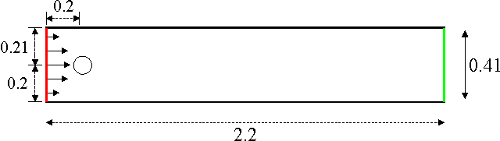
\includegraphics[width=0.8\textwidth]{figures/dfg_geometry.png}
  \caption{Geometría del benchmark DFG 2D-1.}
  \label{fig:dfg2d1_geometry}
\end{figure}

Se consideran las ecuaciones de Navier--Stokes incompresibles (adimensionalizadas con $\rho=1$) en $\Omega$, con viscosidad cinemática $\nu = 0.001$.
\begin{equation}
  \label{eq:dfg1_ns}
  \partial_t u - \nu\,\Delta u + (u\cdot\nabla)u + \nabla p = 0,
  \qquad \nabla\cdot u = 0,
\end{equation}

En las paredes superior e inferior del canal y sobre la frontera del disco se prescribe condición de frontera de no deslizamiento:
\begin{equation}
  \label{eq:dfg1_noslip}
  u=0\quad \text{en } \Gamma_{\mathrm{walls}}\cup \Gamma_{\mathrm{disk}},
\end{equation}
\noindent donde $\Gamma_{\mathrm{walls}} = ([0,2.2]\times\{0\})\cup([0,2.2]\times\{0.41\})$ y $\Gamma_{\mathrm{disk}}=\partial B_r(c)$.

En la entrada $\Gamma_{\mathrm{in}}=\{0\}\times[0,0.41]$ se prescribe un perfil parabólico constante,
\begin{equation}
  \label{eq:dfg1_inflow}
  u(0,y)=\left(\frac{4\,U\,y\,(0.41-y)}{0.41^2},\;0\right),
  \qquad U=0.3,
\end{equation}
\noindent mientras que en la salida $\Gamma_{\mathrm{out}}=\{2.2\}\times[0,0.41]$ se emplea una condición de tipo \textit{do-nothing},
\begin{equation}
  \label{eq:dfg1_outflow}
  \nu\,\partial_{\eta}u - p\,\eta = 0.
\end{equation}

El número de Reynolds se define usando la velocidad media asociada al perfil de entrada. Dado $U=0.3$, se tiene $U_{\mathrm{mean}}=\tfrac{2}{3}\,0.3=0.2$, y tomando como longitud característica el diámetro del cilindro $L=2r=0.1$ se obtiene
\begin{equation}
  \label{eq:dfg1_re}
  Re = \frac{U_{\mathrm{mean}}\,L}{\nu} = \frac{0.2\cdot 0.1}{0.001}=20.
\end{equation}

Para la comparación de resultados se miden las fuerzas de arrastre y sustentación sobre el cilindro. Definiendo el tensor de esfuerzos como
\begin{equation}
  \label{eq:dfg1_stress}
  \sigma := \nu\,\nabla u - pI,
\end{equation}
\noindent las fuerzas se obtienen mediante
\begin{equation}
  \label{eq:dfg1_forces}
  \begin{pmatrix}F_D\\F_L
  \end{pmatrix}
  =\int_{\Gamma_{\mathrm{disk}}}\sigma\,\eta\,ds,
\end{equation}
\noindent donde $\eta$ es el vector normal exterior al círculo (apuntando hacia el fluido). Los coeficientes adimensionales correspondientes se definen como
\begin{equation}
  \label{eq:dfg1_coeffs}
  C_D = \frac{2}{U_{\mathrm{mean}}^2\,L}\,F_D,
  \qquad
  C_L = \frac{2}{U_{\mathrm{mean}}^2\,L}\,F_L.
\end{equation}

Para el caso $Re=20$, el flujo alcanza un estado estacionario. La simulación transitoria se realiza hasta que se satisfaga el criterio de convergencia relativa $\|u^{n+1}-u^n\|_{L^\infty}/(\|u^{n+1}\|_{L^\infty}\Delta t) < 10^{-3}$.


\subsection{Geometría arterial, EAC parametrizable} \label{sec:geom_arterial}

Para estudiar de forma controlada el efecto de la Enfermedad Arterial Coronaria (EAC) en las variables hemodinámicas, se construyen geometrías arteriales bidimensionales con una estenosis simétrica parametrizada. Se usa un parámetro continuo que permite recorrer desde un vaso sano hasta estenosis severas.

Se considera un canal bidimensional de longitud $L$ a lo largo del eje $x$, donde la posición axial está dada por $x \in [0, L]$. El eje central del canal se ubica en $y = R_{\mathrm{in}}$. Para permitir vasos con perfil variable, se fijan dos radios base $R_{\mathrm{in}}$ y $R_{\mathrm{out}}$ en la entrada y la salida. La función que describe el radio de una transición lineal (vaso sano sin estenosis) es
\begin{equation}
  \label{eq:eac_linear_taper}
  R_{\mathrm{taper}}(x)
  := R_{\mathrm{in}} + \left(R_{\mathrm{out}}-R_{\mathrm{in}}\right)\frac{x}{L},
  \qquad x\in[0,L].
\end{equation}

Sobre este perfil base sano, se parametriza el grado de estenosis con una severidad adimensional
\begin{equation}
  \label{eq:eac_severity}
  \eta \in [0,1],
  \qquad
  R_{\min}(\eta)= (1-\eta)\,R_{\mathrm{taper}}(x_m),
\end{equation}
\noindent donde $x_m \in (0,L)$ es la posición axial (centro) de la estenosis y $R_{\min}$ indica el radio interior efectivo en ese punto. De este modo, $\eta=0$ representa un modelo sin alteración de luz y $\eta\to 1$ refleja una constricción de severidad extrema.

El contorno del dominio de flujo está determinado por la pared superior en $y_{\mathrm{top}}(x) = R_{\mathrm{in}} + r(x)$ y la inferior en $y_{\mathrm{bot}}(x) = R_{\mathrm{in}} - r(x)$. El perfil del radio local $r(x)$ se define por tramos continuos. Fuera de la región de estenosis, el canal mantiene su estrechamiento fisiológico natural:
\begin{equation}
  \label{eq:eac_healthy_segments}
  r(x)=R_{\mathrm{taper}}(x),
  \qquad x\in[0,\,x_m-d]\cup[x_m+d,\,L].
\end{equation}

En la región afectada por la estenosis $x\in[x_m-d,\,x_m+d]$, el perfil se genera mediante curvas de Bézier cúbicas. Para asegurar la continuidad y suavidad de la geometría, la interpolacion se establece mediante las siguientes condiciones en los extremos de la región y en el punto de estenosis crítico:
\begin{align*}
  r(x_m-d)=R_{\mathrm{taper}}(x_m-d),
  \qquad
  r(x_m)&=R_{\min},
  \qquad
  r(x_m+d)=R_{\mathrm{taper}}(x_m+d), \\
  r'(x_m-d)=R_{\mathrm{taper}}'(x_m-d),
  \qquad
  r'(x_m)&=R_{\mathrm{taper}}'(x_m),
  \qquad
  r'(x_m+d)=R_{\mathrm{taper}}'(x_m+d).
\end{align*}

La distancia $d$ controla qué tan pronunciada es la transición y se define a partir de un parámetro de pendiente $\alpha>0$ como
\begin{equation}
  \label{eq:eac_d_alpha}
  d = \frac{R_{\mathrm{taper}}(x_m)-R_{\min}}{\alpha}.
\end{equation}

Para implementar este perfil se define la reducción del radio respecto a $R_{\mathrm{taper}}$ como una curva de Bézier cúbica $h(t)$ para el intervalo axial $x \in [x_m - d, x_m]$, donde $t \in [0, 1]$ es el parámetro de la curva. Los puntos de control para la coordenada radial de esta reducción son $h_0 = 0$, $h_1 = 0$, $h_2 = h_{\mathrm{sten}}$ y $h_3 = h_{\mathrm{sten}}$ (siendo $h_{\mathrm{sten}} = R_{\mathrm{taper}}(x_m) - R_{\min}$). El polinomio resultante es:
\begin{equation}
  \label{eq:eac_bezier_h}
  h(t) = (1-t)^3 h_0 + 3(1-t)^2 t h_1 + 3(1-t) t^2 h_2 + t^3 h_3 = h_{\mathrm{sten}}(3t^2 - 2t^3).
\end{equation}

Para la coordenada axial $x(t)$, se emplea otra curva de Bézier que permite controlar la distribución de los elementos de malla mediante un parámetro de tensión $\tau \in [0, 1]$. Los puntos de control axiales son $x_0 = x_m - d$, $x_1 = x_0 + \tau d$, $x_2 = x_m - \tau d$ y $x_3 = x_m$, definiendo el mapeo:
\begin{equation}
  \label{eq:eac_bezier_x}
  x(t) = (1-t)^3 x_0 + 3(1-t)^2 t x_1 + 3(1-t) t^2 x_2 + t^3 x_3.
\end{equation}

Este esquema paramétrico se aplica de forma simétrica para la mitad distal del vaso ($x \in [x_m, x_m+d]$), completando la geometría de la estenosis.

La discretización espacial se realiza con una malla de elementos triangulares. El tamaño local de elemento se adapta según la curvatura de la geometría, refinando alrededor de la estenosis y usando elementos más grandes en las zonas anchas.
\vspace{10pt}

\begin{figure}[htbp]
  \centering
  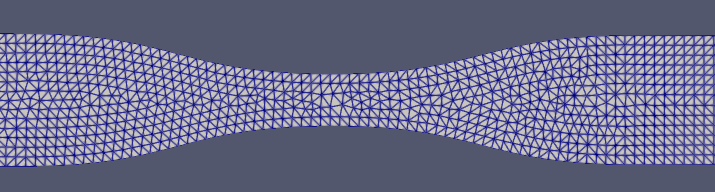
\includegraphics[width=0.8\textwidth]{figures/geometria_arteria.png}
  \caption{Ejemplo de geometría arterial mallada generada con $\eta=0.6$ y  $\alpha = 0.3$.}
  \label{fig:eac_geometria_arteria}
\end{figure}

\subsection{Geometría del lecho microvascular} \label{sec:geom_microvascular}

Para representar la red microvascular, se genera un árbol arterial. La geometría se genera mediante el uso progresivo de bifurcaciones simétricas.

El descenso del radio entre las ramas de cada nivel vascular sigue la ley de Murray \cite{ley_murray}. Asumiendo una bifurcación simétrica y un exponente cúbico estándar $\gamma = 3$, el radio de las ramas hijas $r_{h}$ está dado por el radio de la rama padre $r_{p}$ como:
\begin{equation}
    r_{p}^{3} = 2 r_{h}^{3} \qquad \implies \qquad r_{h} = r_{p} \, 2^{-1/3}.
\end{equation}

La longitud $L$ de los segmentos en red es directamente proporcional a su radio particular gracias a establecer la constante de proporción $\alpha$:
\begin{equation}
    L = \alpha r.
\end{equation}

De igual forma, cada bifurcación establece un mismo ángulo de salida para las ramas hijas, originando finalmente una geometría simetrica y que es consistente con las leyes que rigen el flujo sanguíneo en la microvasculatura.

\begin{figure}[htbp]
  \centering
  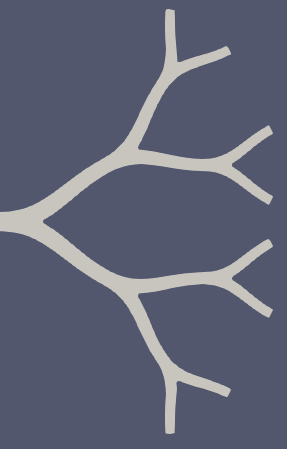
\includegraphics[width=0.35\textwidth, angle=-90]{figures/geom_arbol.png}
  \caption{Geometría de ejemplo para un árbol microvascular con 3 generaciones y relación de aspecto $\alpha = 16$.}
  \label{fig:geom_arbol_ejemplo}
\end{figure}

\subsection{Plataforma para la implementación}

La implementación del modelo numérico se construye sobre un ecosistema de código abierto, priorizando la transparencia y la reproducibilidad de los resultados. Para ello, el desarrollo se basa en la integración de dos librerías principales que permiten abordar la complejidad del problema:

\begin{itemize}
  \item \textbf{FEniCSx:} Se utiliza para la definición de las formas variacionales y su asociación con la geometría del dominio \cite{BarattaEtal2023}. Esta librería permite realizar la discretización y el ensamblaje del sistema de ecuaciones, integrando las condiciones de frontera previamente definidas.

  \item \textbf{PETSc:} Se encarga de resolver los sistemas de ecuaciones resultantes de forma paralela y eficiente \cite{dalcin_parallel_2011}. En este sentido, se emplea el método de Newton para la no linealidad y los métodos de Krylov para la resolución iterativa de los sistemas lineales, garantizando un alto rendimiento computacional.
\end{itemize}

El sistema ha sido diseñado bajo una arquitectura modular de tres capas que separa la física del problema, el método numérico y la orquestación del experimento:

\begin{itemize}
  \item \textbf{Scenario:} Define la física del problema: geometría del dominio, propiedades del fluido ($\mu$, $\rho$), condiciones iniciales y condiciones de frontera (velocidad y presión). Toda nueva geometría o escenario físico se implementa heredando de esta clase abstracta, sobrescribiendo únicamente los métodos \texttt{mesh}, \texttt{bcu}, \texttt{bcp} e \texttt{initial\_velocity}.

  \item \textbf{Solver:} Contiene el esquema numérico para las ecuaciones de Navier--Stokes incompresibles: definición de las formas variacionales, integración temporal y aplicación de condiciones de contorno. Distintos solvers (\textit{estabilizado por bloques}, \textit{Schur}, \textit{LSC}, entre otros) heredan de esta clase y pueden intercambiarse sin modificar el escenario.

  \item \textbf{Simulation:} Actúa como orquestador del experimento: recibe una instancia de \texttt{Scenario} y un \texttt{Solver}, gestiona el bucle temporal, el guardado de resultados y la trazabilidad de los parámetros. Desacopla completamente la lógica de ejecución de la física y del esquema numérico, permitiendo combinar cualquier escenario con cualquier solver y repetir o extender experimentos sin reescribir código.
\end{itemize}

Esta separación en capas permite, por ejemplo, evaluar distintos esquemas numéricos sobre una misma geometría, o probar diferentes condiciones de frontera sin modificar el solver. Para incorporar un nuevo escenario basta con implementar una subclase de \texttt{Scenario}; para añadir un nuevo esquema numérico, una subclase de \texttt{Solver}.


Específicamente para el escenario de la enfermedad coronaria, se combinan las geometrías de la arteria y de la microvasculatura. Este escenario se instancia a partir de archivos de configuración en formato YAML, en donde se especifican todos los parámetros necesarios, que comprenden la elección del escenario, generación de la geometría, parámetros físicos del flujo, parámetros del esquema numérico y elección de condiciones de frontera.

A continuación se detallan todos los parámetros disponibles en el sistema de configuración:

\begin{description}

  \item[\texttt{artery\_params}.] Parámetros de la arteria y la estenosis:\leavevmode
  \begin{itemize}
    \item \texttt{radius\_in} [mm]: Radio de la arteria en la sección de entrada.
    \item \texttt{radius\_out} [mm]: Radio de la arteria en la sección de salida, en el punto de conexión con el árbol microvascular.
    \item \texttt{length} [mm]: Longitud del segmento arterial principal.
    \item \texttt{coupling\_slope} [adimensional]: Pendiente del cono de transición que empalma la arteria con el árbol. Un valor menor produce una transición más gradual.
    \item \texttt{stenosis\_severity} [adimensional]: Severidad de la estenosis ($\eta \in [0, 1]$); $\eta = 0$ representa un vaso sano y $\eta \to 1$ una oclusión extrema.
    \item \texttt{stenosis\_position} [adimensional $\in [0,1]$]: Posición relativa de la estenosis a lo largo del eje axial ($s_m / L$); $0$ es el extremo proximal y $1$ el distal.
    \item \texttt{stenosis\_slope} [adimensional]: Parámetro de pendiente $\alpha$ que controla cuán abrupta es la transición en la zona de estenosis.
  \end{itemize}

  \item[\texttt{tree\_params}.] Parámetros de la microvasculatura:\leavevmode
  \begin{itemize}
    \item \texttt{perf\_pressure} [dyn/cm$^2$]: Presión de perfusión objetivo empleada por \textit{VascuSynth} para dimensionar los radios del árbol ($\approx 133\,322$ dyn/cm$^2$ $\approx$ 100 mmHg).
    \item \texttt{term\_pressure} [dyn/cm$^2$]: Presión objetivo en los nodos terminales empleada por \textit{VascuSynth}.
    \item \texttt{tree\_volume} [ml]: Volumen del dominio cúbico que contiene el árbol microvascular. Determina la escala física de la red.
    \item \texttt{n\_terminal} [entero]: Número de vasos terminales; controla la densidad y la resolución de la red distal.
    \item \texttt{murray\_exponent} [adimensional]: Exponente $\gamma$ de la ley de Murray, que rige la relación de radios en cada bifurcación: $r_\text{parent}^\gamma = r_\text{left}^\gamma + r_\text{right}^\gamma$.
    \item \texttt{mu} [g/(mm$\cdot$s)]: Viscosidad dinámica de la sangre ($\mu \approx 0.0035\,\text{Pa}\cdot\text{s}$). Utilizada por \textit{VascuSynth} para el dimensionamiento hidráulico del árbol.
    \item \texttt{rho} [g/mm$^3$]: Densidad de la sangre ($\rho \approx 0.00106\,\text{g/mm}^3$). Utilizada por \textit{VascuSynth} durante la generación del árbol.
    \item \texttt{wall\_thickening\_severity} [adimensional $\in [0,1]$]: Severidad de la microangiopatía, modelada como engrosamiento de la pared arteriolar y capilar que estrecha el lumen. El factor reduce el radio efectivo de los vasos distales: $r_\text{eff} = r \cdot (1 - \eta_w)$, donde $\eta_w = 0$ representa vasculatura sana y $\eta_w \to 1$ una oclusión completa del lumen. Este parámetro se aplica a los vasos a partir del nivel de árbol definido por \texttt{thickening\_level\_threshold}.
    \item \texttt{thickening\_level\_threshold} [entero]: Nivel del árbol a partir del cual se aplica el engrosamiento de pared. Los vasos en niveles inferiores al umbral (más proximales) no se ven afectados, concentrando la patología en la microvasculatura distal.
    \item \texttt{vessel\_loss\_factor} [adimensional $\in [0,1]$]: Factor de severidad de rarefacción capilar; controla la probabilidad de eliminación de ramas distales del árbol sintético.
    \item \texttt{hyperemia\_dilation\_factor} [adimensional]: Factor multiplicativo de vasodilatación aplicado a los radios del árbol cuando \texttt{hyperemia = true}.
  \end{itemize}

  \item[\texttt{simulation\_params}.] Parámetros del esquema numérico y condiciones de frontera:\leavevmode
  \begin{itemize}
    \item \texttt{T} [s]: Tiempo físico total a simular.
    \item \texttt{dt} [s]: Paso de tiempo $\Delta t$ para la integración temporal.
    \item \texttt{solver}: Esquema numérico empleado. Opciones disponibles: \texttt{stabilized\_staggered}, \texttt{stabilized\_schur}, \texttt{stabilized\_schur\_lsc}, \texttt{solver1}, \texttt{solver2}.
    \item \texttt{mu} [g/(mm$\cdot$s)]: Viscosidad dinámica de la sangre usada en el esquema numérico.
    \item \texttt{rho} [g/mm$^3$]: Densidad de la sangre usada en el esquema numérico.
    \item \texttt{q\_in} [ml/s]: Caudal volumétrico de entrada en condiciones basales. Cuando se prescribe una condición de frontera de velocidad en la entrada, este valor se divide por el área de la sección transversal para obtener la velocidad media $\bar{u} = q_{\mathrm{in}} / A_{\mathrm{in}}$ con la cual se prescribe el perfil de velocidad, ya sea uniforme o parabólico.
    \item \texttt{q\_in\_hyper} [ml/s]: Caudal volumétrico de entrada en hiperemia, utilizado de forma análoga a \texttt{q\_in} cuando \texttt{hyperemia = true}.
    \item \texttt{p\_inlet} [dyn/cm$^2$]: Presión estática prescrita en la entrada, utilizada cuando la condición de frontera de entrada es de tipo presión.
    \item \texttt{p\_terminal} [dyn/cm$^2$]: Presión estática prescrita en las salidas del dominio (arteria o árbol), utilizada cuando la condición de frontera de salida es de tipo presión.
    \item \texttt{bc\_type}: Especifica las condiciones de frontera de entrada y salida:
    \begin{itemize}
      \item \texttt{bc\_type.inlet}: Condición en la entrada. Valores posibles:
        \texttt{velocity\_parabolic} perfil de Poiseuille
        \texttt{velocity\_constant} perfil uniforme,
        \texttt{pressure} presión constante.
      \item \texttt{bc\_type.outlet}: Condición en la salida. Valores posibles:
        \texttt{pressure} presión constante,
        \texttt{none} salida libre,
        \texttt{velocity\_zero} velocidad nula, como una pared.
    \end{itemize}
    \item \texttt{geometry\_type}: Topología de la malla sobre la que se ejecuta la simulación: \texttt{stenosis} (solo arteria), \texttt{tree} (solo árbol microvascular) o \texttt{full} (geometría acoplada completa).
    \item \texttt{hyperemia} [booleano]: Si es \texttt{true}, el escenario usa \texttt{q\_in\_hyper} en lugar de \texttt{q\_in} y activa la vasodilatación del árbol según \texttt{hyperemia\_dilation\_factor}.
  \end{itemize}

  \item[\texttt{matrix}.] Matriz de experimentos:
  Esta sección es opcional y se usa cuando se desea ejecutar un experimento de múltiples escenarios. Cada clave acepta una lista de valores; se calcula el producto cartesiano de todas las listas y se genera un escenario para cada combinación. Los valores de \texttt{matrix} tienen precedencia sobre los declarados en las secciones anteriores para ese escenario concreto.

  Cualquier parámetro de las secciones anteriores puede incluirse en la matriz.
\end{description}


Finalmente, con el objetivo de garantizar la trazabilidad, cada resultado se almacena junto con sus metadatos correspondientes. La información se organiza automáticamente en subcarpetas con una jerarquía que identifica claramente el tipo de simulación, el solver empleado y los parámetros específicos de la ejecución, facilitando el post-procesamiento y los análisis posteriores.


\subsection{Condiciones de frontera}

La presión de entrada $p_\mathrm{in}$ se impone de forma \emph{débil} siguiendo \cite{pressurebc}, lo que permite prescribir simultáneamente condiciones de presión y de velocidad sobre la misma frontera $\Gamma_\mathrm{in}$.

Siguiendo la formulación de \cite{pressurebc}, el término de frontera del tensor de esfuerzos sobre $\Gamma_\mathrm{in}$ en \eqref{momentum_weak} se reemplaza por:

\begin{equation}
  \label{eq:inlet_pressure_bc}
  \int_{\Gamma_\mathrm{in}} p_\mathrm{in} \, (v \cdot n) \, ds.
\end{equation}

Adicionalmente, para mejorar la estabilidad numérica , se decidió prescribir que la componente tangencial de la velocidad en el inlet sea nula, es decir, $u_T = u - (u \cdot n)\,n = 0$ sobre $\Gamma_\mathrm{in}$. Puesto que la frontera de entrada es tratada de forma débil, esta condición no puede imponerse como una restricción de Dirichlet estándar. Por ello, se emplea el \emph{método de Nitsche} \cite{nitsche_original}, que permite imponer de forma consistente y estable condiciones de contorno de tipo Dirichlet de forma débil.

El método de Nitsche para la condición $u_T = 0$ introduce en el residuo los tres términos siguientes \cite{nitsche_ns}:

\begin{equation}
  \label{eq:nitsche_inlet}
  -\int_{\Gamma_\mathrm{in}} \bigl(2\mu\,\varepsilon(u)\cdot n\bigr) \cdot v_T \, ds
  -\int_{\Gamma_\mathrm{in}} \bigl(2\mu\,\varepsilon(v)\cdot n\bigr) \cdot u_T \, ds
  +\frac{\beta_N \mu}{h} \int_{\Gamma_\mathrm{in}} u_T \cdot v_T \, ds,
\end{equation}

\noindent donde $v_T = v - (v \cdot n)\,n$ es la componente tangencial de la función de prueba, $h$ es la longitud característica local del elemento, y $\beta_N > 0$ es el parámetro de penalización de Nitsche. El primer término es la consistencia adjunta de la condición, el segundo garantiza la simetría de la formulación, y el tercero es el término de penalización que asegura la coercividad del problema y el cumplimiento de la condición $u_T = 0$. La formulación resultante es consistente (la solución exacta satisface la forma débil), simétrica e incondicionalmente estable para valores suficientemente grandes de $\beta_N$.

En el \textit{outlet} $\Gamma_\mathrm{out}$, la condición de salida se impone de forma débil prescribiendo una presión $p_{\mathrm{out}}^n$ sobre la frontera. Esto se logra de la misma forma que con a presion en la frontera de entrada, añadiendo el término que reemplaza al término de tracción natural del tensor de esfuerzos sobre $\Gamma_\mathrm{out}$:
\begin{equation}
  \label{eq:outlet_pressure_weak}
  \int_{\Gamma_\mathrm{out}} p_{\mathrm{out}}^n \, (v \cdot n) \; ds.
\end{equation}

No obstante, la condición de presión impuesta débilmente en el \textit{outlet} puede inducir inestabilidades numéricas cuando el flujo local se invierte, por ejemplo, al paso de vórtices o en regimen pulsátil. En esos instantes, el flujo que retrocede introduce energía cinética al sistema, lo que puede llevar a la divergencia del método \cite{bc_backflow_hemo,modified_bc_hemo}. Para suprimir este fenómeno, se añade el término de penalización de \textit{backflow} propuesto en \cite{bc_backflow_hemo}:
\begin{equation}
  \label{eq:backflow_term}
  -\int_{\Gamma_\mathrm{out}} \beta_b \, \rho \, (u^{n-1} \cdot n)_- \; (u \cdot v) \; ds,
\end{equation}
\noindent donde $\beta_b > 0$ es el parámetro de penalización y
\begin{equation*}
  (u^{n-1} \cdot n)_- \;=\; \tfrac{1}{2}\bigl(u^{n-1}\cdot n \;-\; |u^{n-1}\cdot n|\bigr)
\end{equation*}
es la parte negativa de la velocidad normal evaluada en el paso anterior, de modo que el término solo penaliza donde el flujo retrocede.

La elección de $p_{\mathrm{out}}^n$ requiere especial atención. La presión en la salida del dominio no es independiente de la geometría simulada: a mayor severidad de la estenosis, mayor es el gradiente de presión a través del vaso, y la presión en el \textit{outlet} también depende de la resistencia hidráulica del territorio distal (el árbol microvascular) que no se simula explícitamente por completo. En consecuencia, la presión de salida no puede prescribirse directamente a partir de datos conocidos a priori.

Una elección consistente con la fisiología es suponer una relación lineal entre el flujo volumétrico $Q$ y la presión en el \textit{outlet}:
\begin{equation}
  \label{eq:resistance_bc}
  p_{\mathrm{out}} = R \cdot Q,
\end{equation}
\noindent donde $R$ es la resistencia vascular periférica del lecho distal. Esta condición modela el dominio no simulado aguas abajo del \textit{outlet} y es independiente de la geometría interna del dominio principal. La relación \eqref{eq:resistance_bc} es consistente con un flujo de Poiseuille completamente desarrollado \cite{mcdonalds_fisiology}, donde la caída de presión es proporcional al caudal. Esta suposición es pertinente en la microvasculatura, dado que los radios de los vasos capilares son muy pequeños, el número de Reynolds local es bajo y el flujo es efectivamente laminar y completamente desarrollado \cite{outflow_resistance}.

En la implementación se adopta un acoplamiento explícito, la presión de salida en el paso $n$ se calcula con el caudal del paso anterior,
\begin{equation}
  \label{eq:resistance_explicit}
  p_c^n = R \cdot Q^{n-1}, \qquad Q^{n-1} = \int_{\Gamma_\mathrm{out}} u^{n-1} \cdot n \; ds.
\end{equation}

\subsubsection{Resistencia para el árbol microvascular}

Para el escenario acoplado de la estenosis con el árbol microvascular explícito, la condición de frontera de resistencia prescrita en los terminales del árbol debe reflejar la resistencia periférica total ($R_{\mathrm{target}}$) descontando la resistencia propia de la parte de la red microvascular que sí es simulada de forma explícita ($R_{\mathrm{arbol}}$). Por lo tanto, el valor de resistencia a prescribir en las fronteras terminales del árbol es:
\begin{equation}
  R_{\mathrm{out}} = R_{\mathrm{target}} - R_{\mathrm{arbol}}.
\end{equation}

El valor de $R_{\mathrm{arbol}}$ se puede aproximar de forma analítica aprovechando que conocemos el radio de los vasos en cada nivel gracias a la ley de Murray. Para este desarrollo, el perfil de flujo de Poiseuille entre 2 placas tiene varias limitaciones, por lo que asumimos el perfil de flujo de Poiseuille para conductos cilíndricos. Bajo estas condiciones, la resistencia hidráulica de un vaso de radio $r$ y longitud $L$ viene dada por:
\begin{equation}
  R = \frac{8 \mu L}{\pi r^4}
\end{equation}

En la generación de la geometria del árbol microvascular, la longitud del vaso en cada nivel mantiene una proporcion fija con el radio, de manera que $L = \alpha r$. Al sustituir esta definición, obtenemos que la resistencia particular de un vaso en el primer nivel del árbol (de radio $r_0$) es:
\begin{equation}
  R_0 = \frac{8 \mu \alpha}{\pi r_0^3}
\end{equation}

Luego, la ley de Murray especifica que para una bifurcación simétrica se cumple que $r_{\mathrm{padre}}^3 = 2 r_{\mathrm{hija}}^3$, por lo que el radio para cualquier rama en un nivel del árbol $j$ es:
\begin{align}
  r_{\mathrm{j}} &= r_{\mathrm{j-1}} \, 2^{-1/3} \nonumber \\
  r_j &= r_0 \prod_{i=1}^{j} 2^{-1/3} \nonumber \\
  r_j &= r_0 \, 2^{-j/3}
\end{align}

Con esto, la resistencia local de un vaso en el nivel $j$ es:
\begin{equation}
  R_{\mathrm{vaso}, j} = \frac{8 \mu \alpha}{\pi r_j^3} = \frac{8 \mu \alpha}{\pi \left(r_0 \, 2^{-j/3}\right)^3} = R_0 \, 2^j
\end{equation}

Hay que tener en cuenta que en cada nivel del árbol, existen $2^j$ vasos idénticos dispuestos en paralelo. Por lo tanto, el caudal total del sistema ($Q_{\mathrm{total}}$) se divide equitativamente y cada vaso transporta una fracción del flujo: $Q_j = Q_{\mathrm{total}} / 2^j$.

Al ser un sistema simétrico, la caída de presión $\Delta P_j$ al atravesar el nivel $j$ es la misma en cualquier vaso: $\Delta P_j = R_{\mathrm{vaso}, j} \cdot Q_j$. Sustituyendo la porción de caudal correspondiente observamos que:
\begin{equation} \label{eq:deltap_nivel}
  \Delta P_j = R_{\mathrm{vaso}, j} \left( \frac{Q_{\mathrm{total}}}{2^j} \right) = \left( \frac{R_{\mathrm{vaso}, j}}{2^j} \right) Q_{\mathrm{total}}
\end{equation}

La resistencia de un nivel entero se define como la razón entre su caída de presión y el caudal total del sistema: 
\begin{equation} \label{eq:resistencia_nivel}
  R_{\mathrm{nivel}, j} = \frac{\Delta P_j}{Q_{\mathrm{total}}}
\end{equation}

Reemplazando la caida de presión \eqref{eq:deltap_nivel} se obtiene:
\begin{equation}
  R_{\mathrm{nivel}, j} = \frac{R_{\mathrm{vaso}, j}}{2^j} = \frac{R_0 \, 2^j}{2^j} = R_0
\end{equation}

La resistencia total del árbol se obtiene sumando las resistencias de cada nivel:
\begin{equation}\label{eq:resistencia_arbol}
  R_{\mathrm{arbol}} = \sum_{j=0}^{N_{\mathrm{gen}}-1} R_{\mathrm{nivel}, j} = \sum_{j=0}^{N_{\mathrm{gen}}-1} R_0  = N_{\mathrm{gen}} \frac{8 \mu \alpha}{\pi r_0^3}
\end{equation}


\subsection{Simulación}

\subsubsection{Parámetros de la simulación}

La geometría del segmento arterial se parametrizó con base en medidas morfométricas de la arteria descendente anterior izquierda (LAD) obtenidas mediante angiogramas coronarios y angiografía de rayos X. La longitud del segmento se fijó en $L = 138\,\text{mm}$, valor que cae dentro del rango de $72.46$--$144.78\,\text{mm}$ reportado en \cite{lad_length}. El radio de entrada se estableció en $R_{\mathrm{in}} = 1.57\,\text{mm}$, mientras que el radio de salida se fijó en $R_{\mathrm{out}} = 1.20\,\text{mm}$, de acuerdo a los valores reportados en \cite{lad_diameter}.

La presión de entrada se fijó en $p_{\mathrm{in}} = 75\,\mathrm{mmHg}$, valor representativo de la presión diastólica normal \cite{blood_pressure_aha}. Para las propiedades del fluido se adoptaron valores estándar de la sangre: densidad $\rho = 1.060\times10^{-3}\,\mathrm{g/mm^3}$ y viscosidad dinámica $\mu = 3.5\times10^{-3}\,\mathrm{Pa\cdot s}$. Para el esquema numérico se seleccionó un paso de tiempo $\Delta t = 10^{-4}\,\mathrm{s}$, un parámetro de penalización de \textit{backflow} $\beta_b = 0.6$ y un parámetro de Nitsche $\beta_N = 100$.

Para el árbol microvascular, se decidió generar $3$ niveles. Esta elección se fundamenta en simulaciones preliminares que mostraron que, a partir de dicho nivel, el número de Reynolds es muy bajo ($Re < 5$) y el flujo entra en un régimen laminar y completamente desarrollado. En consecuencia, la dinámica de flujo en el resto del árbol vascular puede aproximarse adecuadamente de forma analítica.

Por otro lado, el valor de la resistencia de salida $R$ se estimó a partir de mediciones promedio de presión y flujo en pacientes sanos. Según \cite{velocity_lad}, la velocidad de flujo media en la LAD a nivel distal es de $v_{\mathrm{media}} = 280\,\mathrm{mm/s}$. La velocidad media sobre un diámetro transversal de altura $h$ se expresa como:
\begin{equation*}
  v_{\mathrm{media}} = \frac{1}{h} \int_0^h v(y) \; dy.
\end{equation*}

Asumiendo que el flujo es laminar y, por lo tanto, la velocidad es normal a la sección transversal, podemos relacionar el caudal $Q$ con la velocidad media de la siguiente manera:
\begin{equation}
  Q = \int_0^h (v(y) \cdot n) \; dy = \int_0^h v(y) \; dy = v_{\mathrm{media}} \cdot h.
\end{equation}

Entonces, al considerar un diámetro $h = 2.41\,\mathrm{mm}$, el flujo resulta en $Q = 280\,\mathrm{mm/s} \cdot 2.41\,\mathrm{mm} = 674.8\,\mathrm{mm^2/s}$.

Teniendo en cuenta la presión diastólica normal previamente seleccionada ($p = 75\,\mathrm{mmHg}$), la cual se puede expresar en el sistema de unidades empleado en la simulación asumiendo que $1\,\mathrm{mmHg} \approx 133\,\mathrm{Pa}$, se obtiene una presión efectiva de $p \approx 9310\,\mathrm{Pa}$, lo que equivale a $9310\,\mathrm{g/(mm \cdot s^2)}$. Con base en la relación general $p = R \cdot Q$, la resistencia a nivel distal de la arteria se estima como:
\begin{equation}
  R = \frac{p}{Q} = \frac{9310\,\mathrm{g/(mm \cdot s^2)}}{674.8\,\mathrm{mm^2/s}} \approx 13.79\,\mathrm{g \cdot s/mm}.
\end{equation}.

\subsubsection{Convergencia de malla}

Se realizó un estudio de convergencia de malla con el fin de determinar una resolución suficientemente refinada para las simulaciones posteriores. 

Se adoptó una estrategia de refinamiento hp, donde se reduce el tamaño de los elementos de la malla, al tiempo que se aumenta el orden de los polinomios de aproximación, hasta lograr convergencia de la solución. La convergencia se evaluó sobre el cambio en la norma $L^2$ tanto de la velocidad como de la presión entre dos simulaciones consecutivas.  

Se analizó la geometria completa, estenosis y árbol microvascular con tres niveles; se consideraron tres escenarios: obstrucción leve (25\%), moderada (50\%) y severa (75\%). Se inicío con polinomios de grado uno y elementos de tamaño $0.3$ mm y se obtuvo convergencia (cambio $< 1\%$) con polinomios de grado dos y elementos de tamaño $0.15$ mm. 


\subsubsection{Impacto de la ubicación axial de la estenosis}

Con el objetivo de evaluar si la ubicación de la estenosis a lo largo de la arteria tiene algún impacto sobre los índices diagnósticos o el flujo en el árbol vascular, se ejecutaron escenarios de simulación específicos. Se seleccionaron tres niveles de severidad de la estenosis ($25\%$, $50\%$ y $75\%$), cada uno evaluado en dos posiciones axiales distintas: una ubicación proximal al inicio de la arteria ($25\%$ de la longitud total) y una ubicación distal hacia el final de la misma ($75\%$ de la longitud).

\subsubsection{Impacto de la forma de la estenosis}

Para investigar de qué manera la morfología de la lesión afecta las variables hemodinámicas y los índices diagnósticos, se evaluó el impacto de la forma geométrica de la oclusión. En particular, se buscó determinar si existe un comportamiento diferente entre una estenosis prolongada y una más corta, si la forma abrupta de la lesión supone un factor importante, o si el impacto sobre el flujo vascular está regido principalmente por el nivel de severidad.

Con este propósito, se plantearon $9$ escenarios de simulación correspondientes a todas las combinaciones posibles de tres niveles de severidad ($\eta \in \{0.25, 0.5, 0.75\}$) y tres parámetros de pendiente ($\alpha \in \{0.05, 0.15, 0.3\}$).

\begin{figure}[htbp]
  \centering
  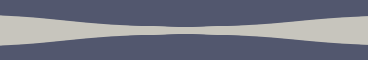
\includegraphics[width=0.9\textwidth]{figures/stenosis_severity75_slope005.png} \\
  \vspace{1cm}
  
\includegraphics[width=0.9\textwidth]{figures/stenosis_severity75_slope03.png}
  \caption{Comparación de formas de estenosis: gradual con severidad del 75\% y pendiente de 0.05 (arriba) y abrupta con severidad del 75\% y pendiente de 0.3 (abajo).}
  \label{fig:comparacion_forma_estenosis}
\end{figure}

\subsubsection{Por decidir (bla bla resistencia severidad indices diagnosticos)}
- explicacion calculo FFR/CFR

Para evaluar el impacto hemodinámico de la disfunción microvascular (DMV), se planteó un análisis variando la resistencia periférica desde un estado sano hasta uno patológico. Esta transición simula las dos alteraciones principales de la DMV: la rarefacción capilar (pérdida de capilares) y el engrosamiento de pared (reducción uniforme de radios) \cite{concenso_minoca_arg}. 

En primer lugar, se asume un árbol microvascular de referencia (sano). Para establecer su profundidad, se determinó el número de generaciones necesarias para que los vasos terminales alcancen dimensiones capilares (diámetro entre $5$ y $10\,\mu\mathrm{m}$) \cite{circulacion_capilar}. Evaluando la ley de Murray $r_j = r_0 \, 2^{-j/3} \le 0.0025\,\mathrm{mm}$ desde el vaso principal $r_0 = 1.2\,\mathrm{mm}$, se alcanzan las capilares en la generación $27$ ($r_{27} \approx 2.34\,\mu\mathrm{m}$). Estableciendo entonces $N_{\mathrm{gen}} = 27$, la resistencia de este árbol sano ($R_{\mathrm{geom}}^{\mathrm{sano}}$) se evalúa usando \eqref{eq:resistencia_arbol} y es igual a $27 R_0$.

Posteriormente, se simulan las dos alteraciones patológicas en la topología para obtener la resistencia enferma ($R_{\mathrm{geom}}^{\mathrm{enfermo}}$):

Primero se modela el engrosamiento de pared utilizando el porcentaje de área transversal ocupada por la pared respecto al área total del vaso. En un estudio de arteriolas coronarias intramiocárdicas \cite{dmv_remodelation_lumen}, los pacientes con presión arterial normal estaban en promedio en $66\%$, mientras que las de pacientes hipertensos en $69.9\%$. Definiendo el área luminal como el complemento ($100\% - \text{área de pared}$), el área de flujo en sujetos sanos es del $34\%$, mientras que en hipertensos se reduce al $30.1\%$. El estudio muestra que el radio externo se mantiene constante, por lo que el factor por el que se reduce el radio interno en pacientes enfermos es: $\beta = \sqrt{\frac{0.301}{0.340}} \approx 0.9409$. 
  
Luego se modela la rarefacción, los valores normales de densidad capilar varían entre $2500$ y $3000\,\mathrm{capilares/mm^2}$. Bajo ciertas patologías, la densidad disminuye a unos $1500 - 2000\,\mathrm{capilares/mm^2}$ \cite{rarefaction}, lo que equivale a una reducción de capilares ($\xi$) de entre un $20\%$ y $40\%$. Para reproducirlo matemáticamente, el número de ramas se reduce multiplicando el número de vasos en paralelo por el factor $(1-\xi)$. Esta disminución se aplica exclusivamente sobre las generaciones correspondientes a la microcirculación (niveles $j \ge N_{\mathrm{micro}}$).

Aplicando la constricción luminal (que aumenta la resistencia tubular por un factor de $1/\beta^4$) y la reducción de capilares (que disminuyen el flujo en paralelo por $1-\xi$), la resistencia del arbol representativo de DMV es:
\begin{equation}
  R_{\mathrm{geom}}^{\mathrm{enfermo}} = \sum_{j=0}^{N_{\mathrm{micro}}-1} \frac{R_0}{\beta^4} + \sum_{j=N_{\mathrm{micro}}}^{N_{\mathrm{gen}}-1} \frac{R_0}{\beta^4 (1-\xi)}
\end{equation}

Con estas ecuaciones, el factor de aumento resistivo ($k_R$) se evalúa como:
\begin{equation}
  k_R = \frac{R_{\mathrm{geom}}^{\mathrm{enfermo}}}{R_{\mathrm{geom}}^{\mathrm{sano}}}
\end{equation}

Para evaluar la severidad máxima, se determinó el inicio de la red capilar ($N_{\mathrm{micro}}$) como el nivel donde el radio luminal es $\leq 10\,\mu\mathrm{m}$ \cite{circulacion_capilar}. Evaluando $r_0 \, 2^{-j/3} \le 0.01\,\mathrm{mm}$ con $r_0 = 1.2\,\mathrm{mm}$, se obtiene que la rarefacción inicia en $N_{\mathrm{micro}} = 21$.

Se adoptaron los parámetros extremos para establecer la cota patológica máxima: un factor de contracción luminal $\beta = 0.9409$ (incrementando la resistencia tubular por el factor $1/\beta^4 \approx 1.275$) y una pérdida de densidad capilar del $40\%$ ($\xi = 0.40$, con una vascularidad remanente del $60\%$).

Sustituyendo estos parámetros para las $N_{\mathrm{gen}} = 27$ generaciones y $N_{\mathrm{micro}} = 21$:
\begin{equation}
  k_R = \frac{\frac{R_0}{\beta^4} \left[ 21 + \frac{27-21}{0.6} \right]}{27 R_0} \approx \frac{1.275 \left[ 21 + 10 \right]}{27} \approx 1.464
\end{equation}

Escalando la resistencia basal, la condición de frontera para el árbol enfermo resulta en:
\begin{equation} \label{eq:r_enfermo}
  R_{\mathrm{enfermo}} = R_{\mathrm{base}} \cdot 1.464 = 13.79 \cdot 1.464 \approx 20.19\,\mathrm{g \cdot s/mm}
\end{equation}

De esta manera, el rango de resistencias a explorar para determinar el impacto de la enfermedad es $[13.79, 20.19]\,\mathrm{g \cdot s/mm}$.

- experimento relacion severidad/pendiente/resistencia -> FFR/CFR


\section{Resultados}

\subsection{Benchmarks de validación} \label{sec:resultados_validacion}

\subsubsection{Flujo en cavidad inducida por tapa (Lid-Driven Cavity)}

Como paso previo a la comparación con los datos de referencia, se realizó un estudio de convergencia de malla con el fin de determinar una resolución suficientemente refinada. Se simuló hasta llegar a el estado estacionario, con mallas uniformes de $N \times N$ elementos, con $N \in \{20, 30, 40, 50, 60, 70, 80, 90, 100\}$, y se registró la norma $L^2$ de la velocidad y de la presión en cada caso. Los resultados se muestran en la \cref{fig:ldc_convergencia_re1000}.

\begin{figure}[htbp]
  \centering
  \captionsetup{justification=centering}
  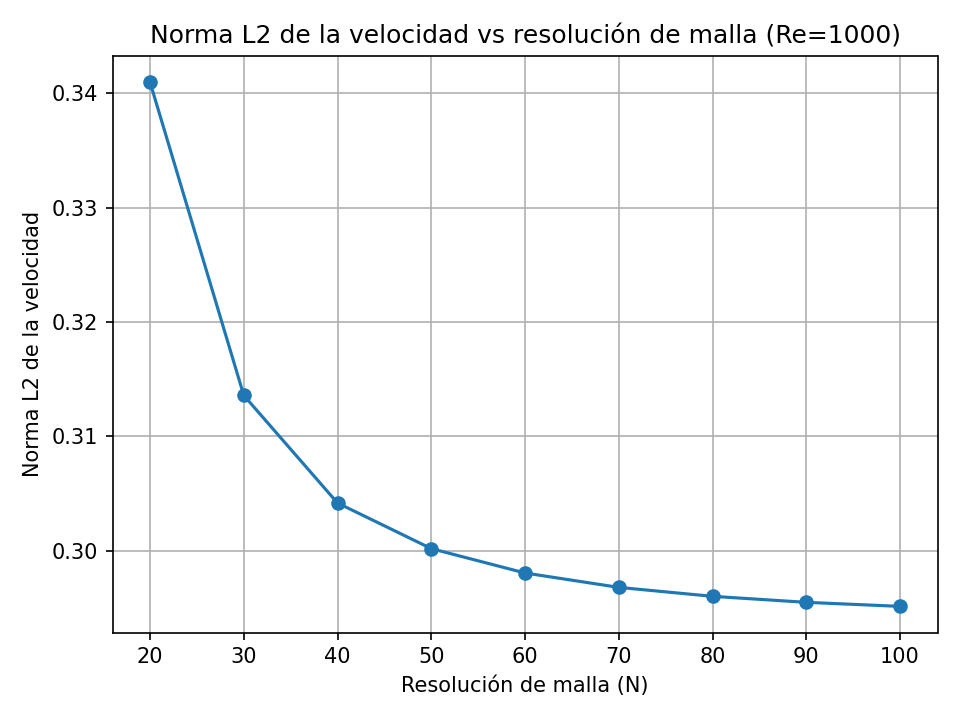
\includegraphics[width=0.48\textwidth]{figures/norma_velocidad_lid_driven1000.png}
  \hfill
  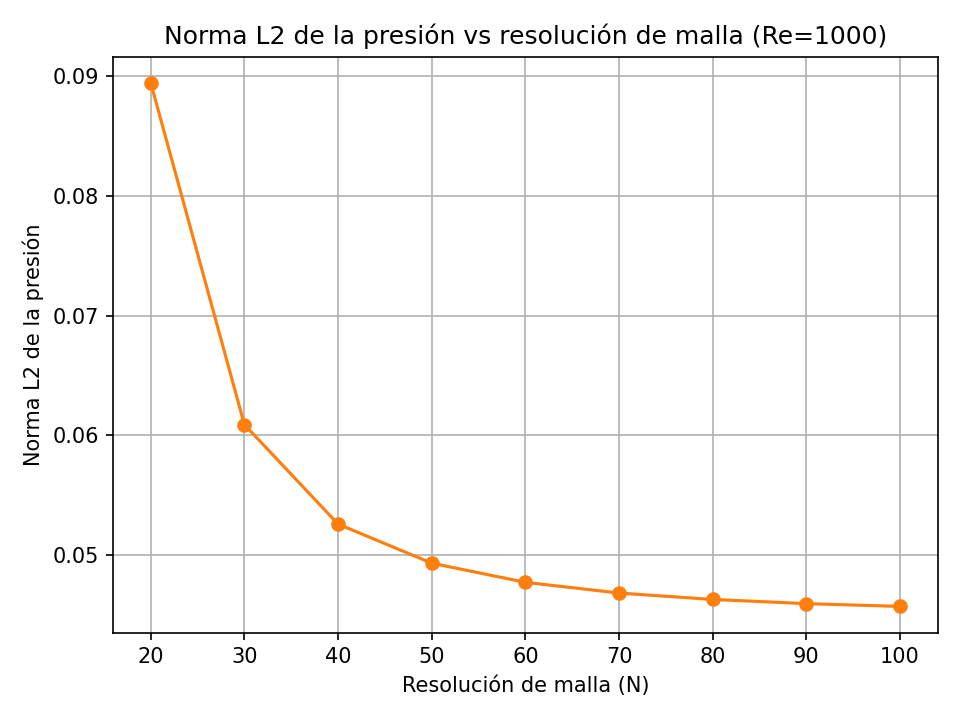
\includegraphics[width=0.48\textwidth]{figures/norma_presion_lid_driven1000.png}
  \caption{Convergencia de malla para el benchmark de el \cref{sec:ldc}: norma $L^2$ de la velocidad (izquierda) y de la presión (derecha) en función de la resolución de malla $N$.}
  \label{fig:ldc_convergencia_re1000}
\end{figure}

Ambas normas decrecen monótonamente al refinar la malla y se estabilizan a partir de $N=90$. En particular, la variación relativa entre las dos últimas mallas consecutivas ($N=90$ y $N=100$) fue inferior al $1\%$ en ambas variables: $0{,}11\%$ para la velocidad y $0{,}5\%$ para la presión. Este criterio confirma la convergencia de la solución y justifica el uso de $N=100$ como malla de referencia para las comparaciones posteriores.

La \cref{fig:ldc_lineplot_re1000} muestra la comparación de la componente $x$ de la velocidad a lo largo de la recta $\{(x,y) : x=0.5; 0 \le y \le 1\}$ frente a los datos de referencia reportados por Ghia et al. \cite{ghia_high-re_1982} para $Re=1000$, utilizando la malla de $N=100$.

\begin{figure}[htbp]
  \centering
  \captionsetup{justification=centering}
  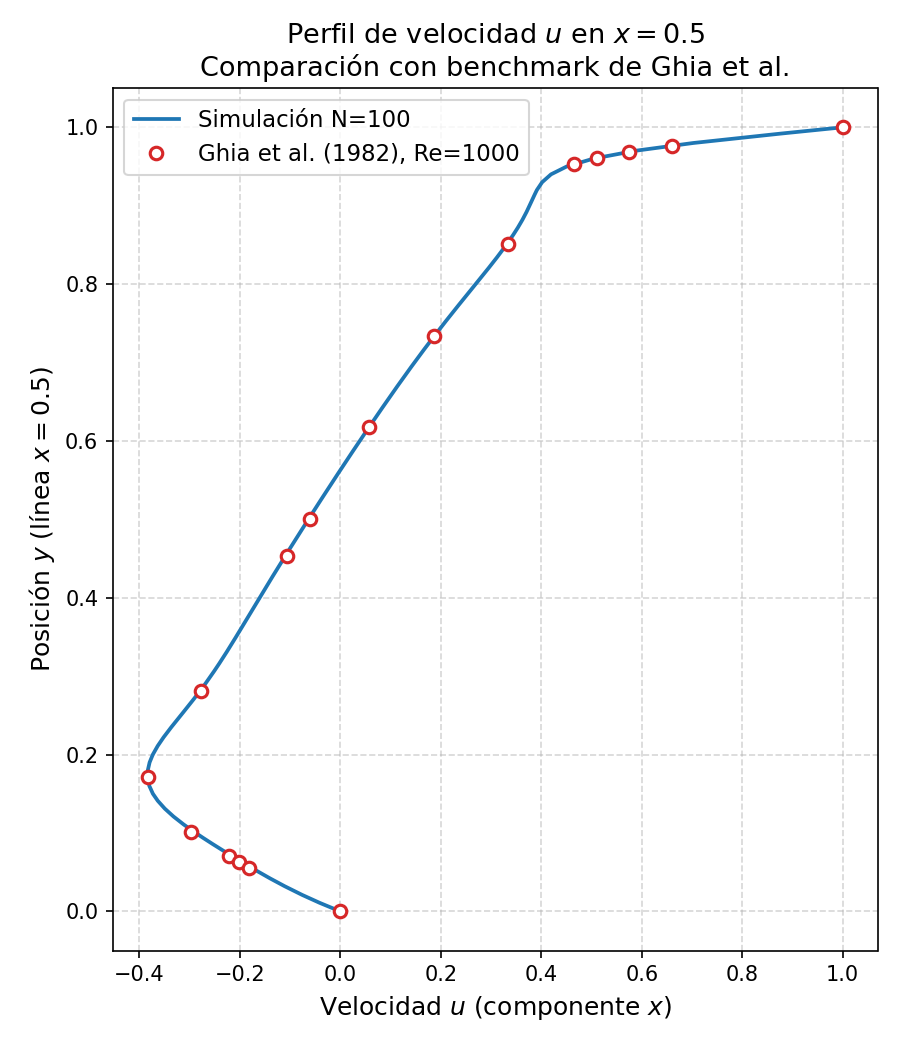
\includegraphics[width=0.6\textwidth]{figures/ghia_comparison.png}
  \caption{Componente $x$ de la velocidad en la recta $x=0.5$ para el benchmark de el \cref{sec:ldc} con $N=100$, frente a los datos de \cite{ghia_high-re_1982}.}
  \label{fig:ldc_lineplot_re1000}
\end{figure}

La curva simulada reproduce con fidelidad el perfil de referencia, capturando correctamente tanto las zonas de recirculación cercanas a las esquinas como el máximo de velocidad en la región central. Esto confirma la validez del solver para este número de Reynolds.

Adicionalmente, en la \cref{fig:ldc_streamlines_re1000} se contrastan cualitativamente los mapas de líneas de corriente. Ambos muestran un vórtice primario centrado ligeramente por encima del centro geométrico, así como dos vórtices secundarios en las esquinas inferiores y otro en la superior izquierda. El patrón obtenido en la simulación concuerda cualitativamente con la referencia.

\begin{figure}[htbp]
  \centering
  \captionsetup{justification=centering}
  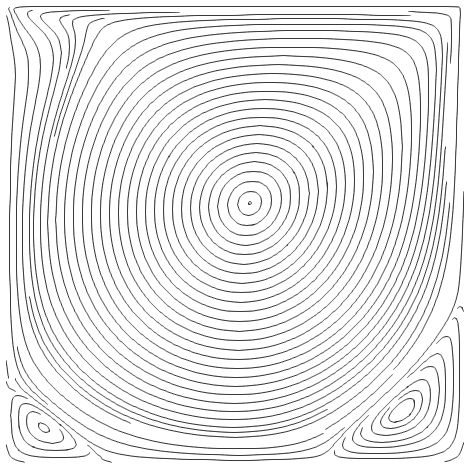
\includegraphics[width=0.48\textwidth]{figures/streamlines_simulation.png}
  \hfill
  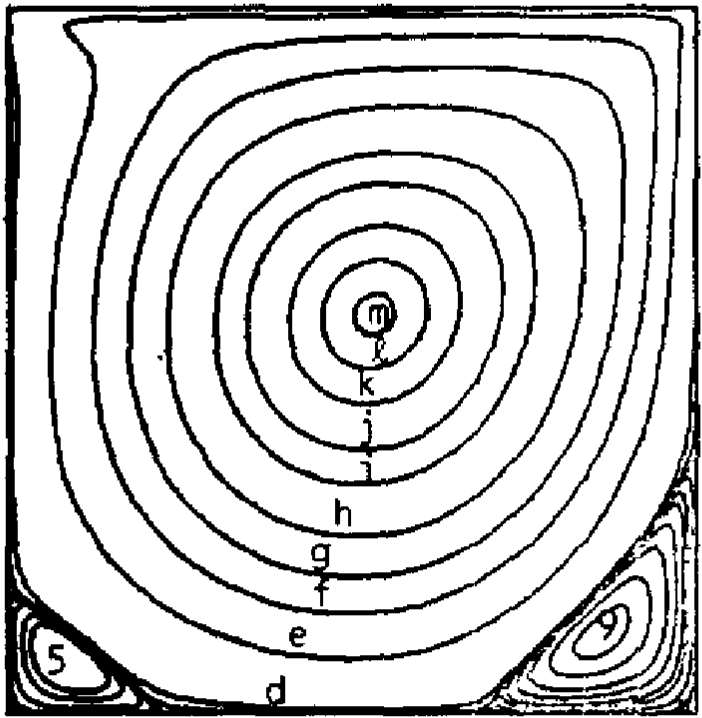
\includegraphics[width=0.465\textwidth]{figures/streamlines_ghia.png}
  \caption{Líneas de corriente para el benchmark de el \cref{sec:ldc}: simulación con $N=100$ (izquierda) y referencia de \cite{ghia_high-re_1982} (derecha).}
  \label{fig:ldc_streamlines_re1000}
\end{figure}

\subsubsection{Flujo alrededor de un cilindro (Benchmark DFG 2D-1)} \label{sec:dfg_results}

Como paso previo a la validación con los valores de referencia, se realizó un estudio de convergencia de malla para determinar una resolución suficientemente refinada en las cercanías del obstáculo. Se simuló hasta llegar a estado estacionario para distintas resoluciones, $res \in \{0.01, 0.005, 0.0025\}$, ajustando el refinamiento local alrededor del cilindro y tanto para interpolación con polinomios de primer orden como de segundo orden. En cada caso se registraron los coeficientes de arrastre ($C_D$) y sustentación ($C_L$). Los resultados se muestran en la \cref{fig:dfg1_convergencia}.

\begin{figure}[htbp]
  \centering
  \captionsetup{justification=centering}
  % 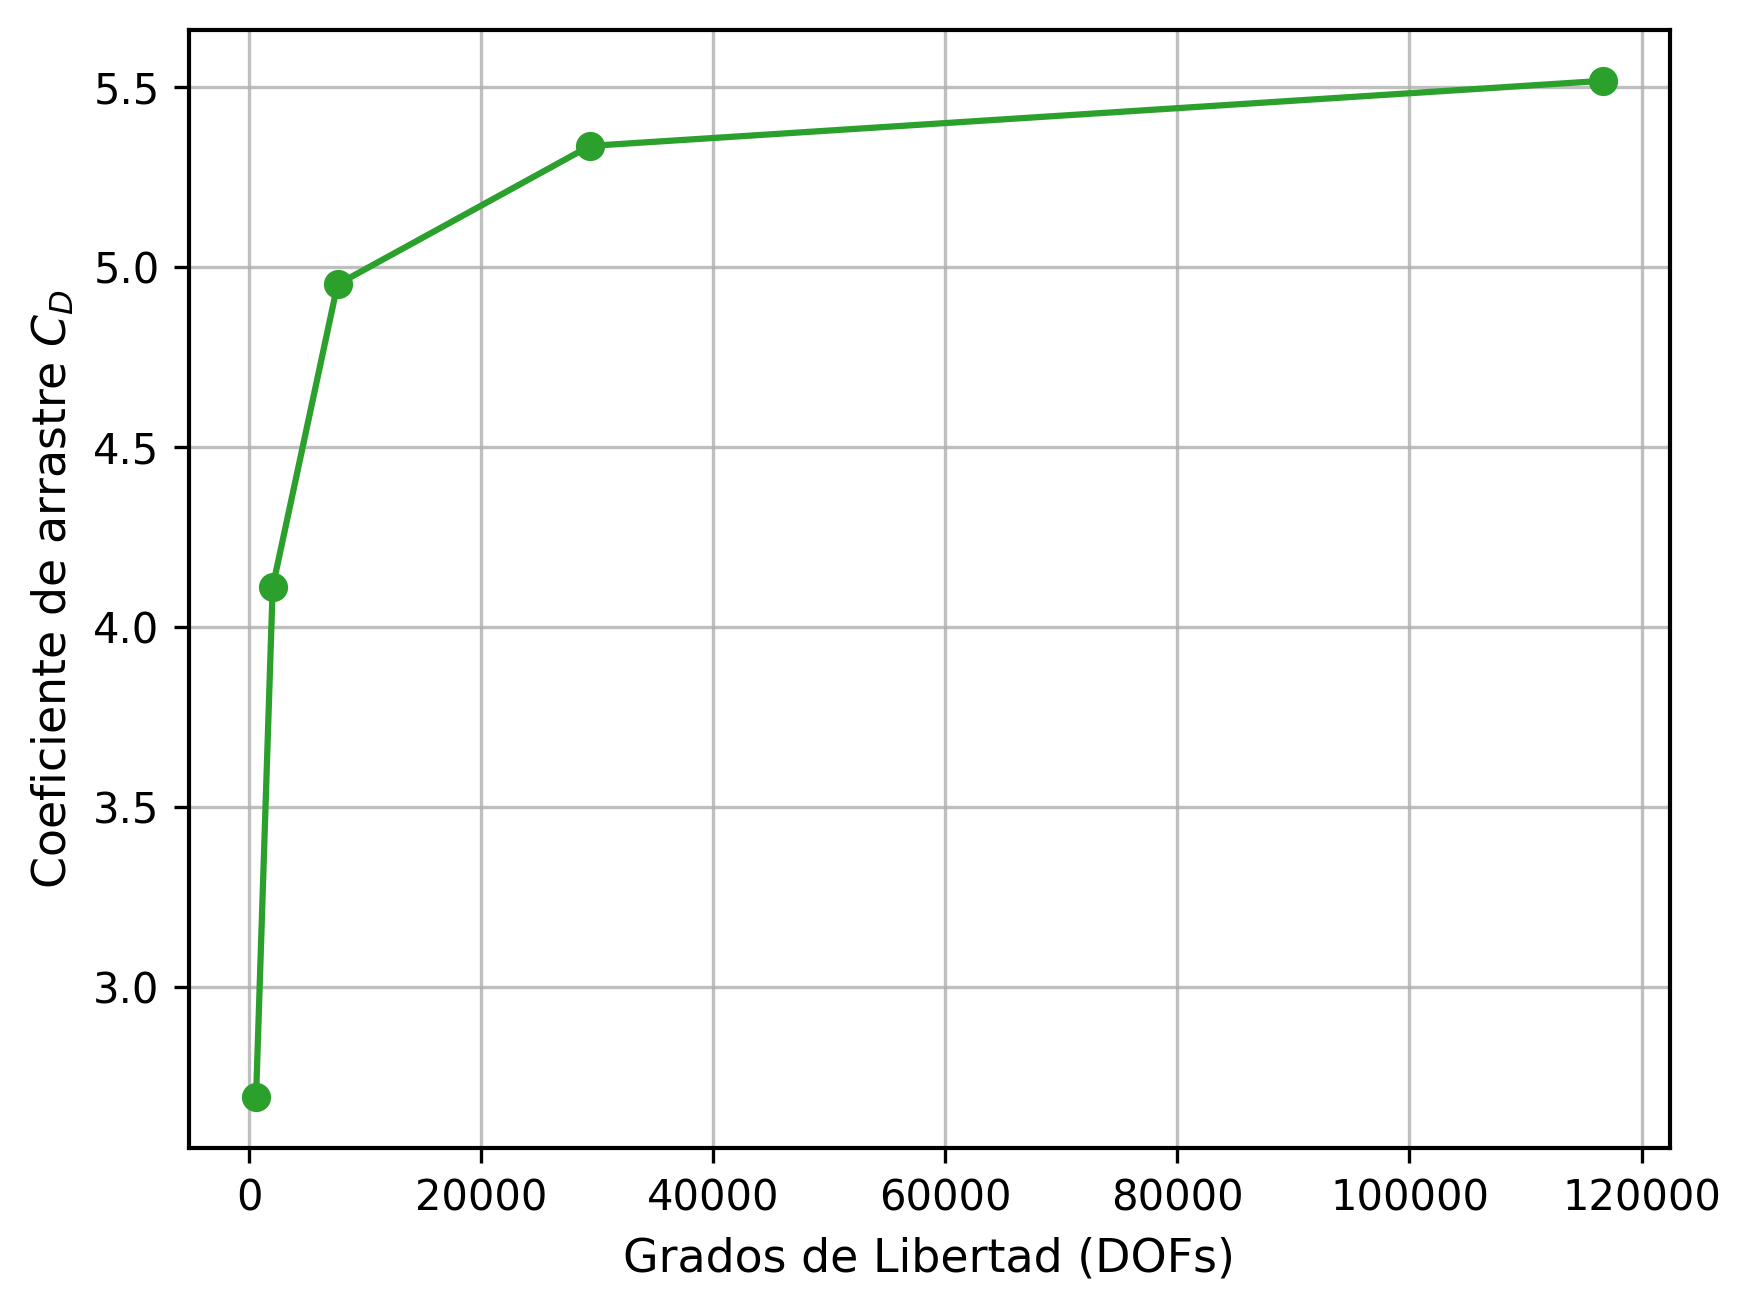
\includegraphics[width=0.48\textwidth]{figures/dfg1_drag_convergence.png}
  % \hfill
  % 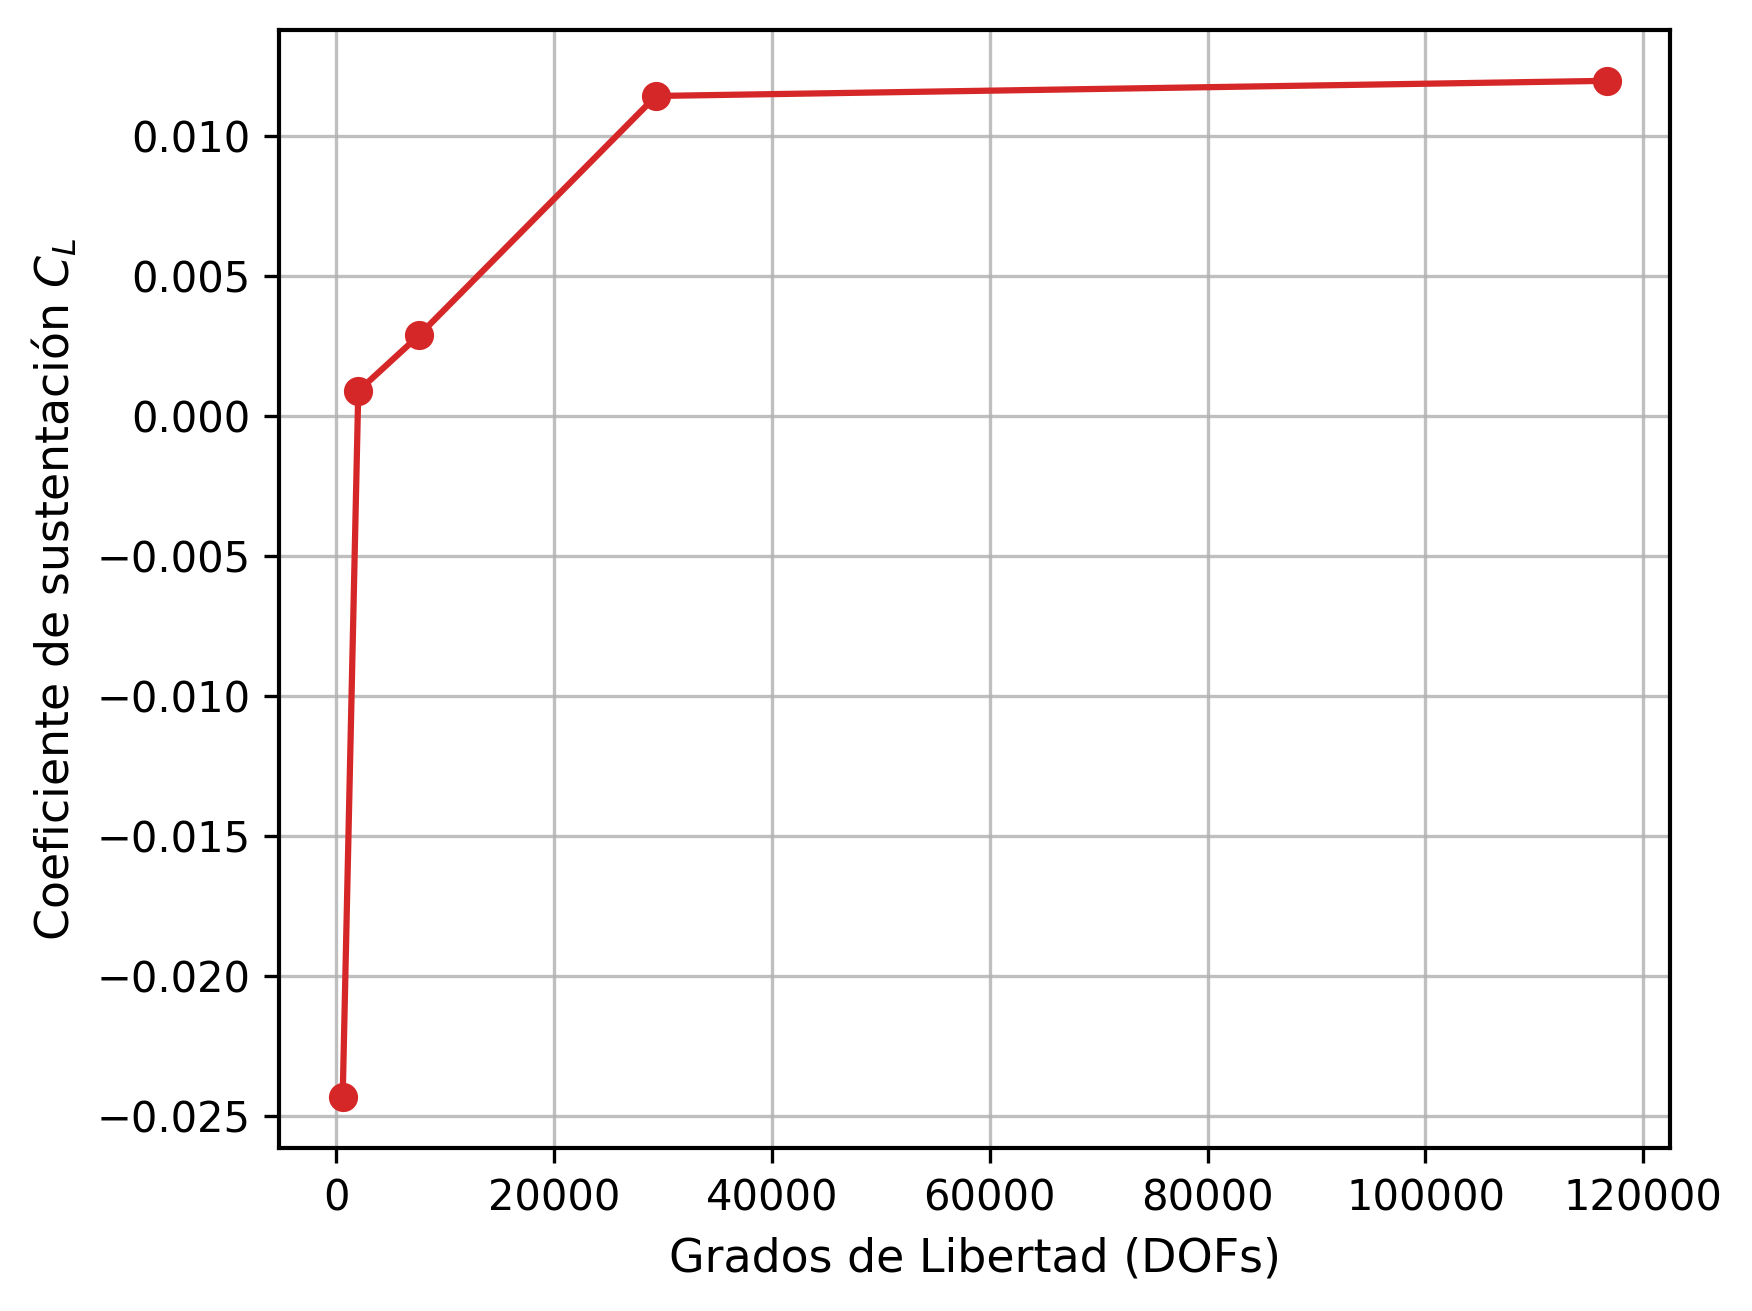
\includegraphics[width=0.48\textwidth]{figures/dfg1_lift_convergence.png}
  \caption{Convergencia de malla para el benchmark DFG 2D-1: coeficiente de arrastre $C_D$ (izquierda) y de sustentación $C_L$ (derecha) en función del parámetro de resolución $res$.}
  \label{fig:dfg1_convergencia}
\end{figure}

Se observa que ambos coeficientes convergen monótonamente hacia los valores tabulados a medida que se reduce el valor de $res$. La variación relativa entre las mallas de $res=0.007$ y $res=0.005$ fue inferior al $0.5\%$, lo que justifica el uso de $res=0.005$ como resolución de referencia para las comparaciones presentadas a continuación.



\subsection{Analisis descriptivo de parametros hemodinamicos}

un analiss descriptivo de las variables tanto en stenosis y en arbol:

en stenosis:
- velocidad
- presion
- wss
-streamlines
- vorticidad


en arbol:
- simetria
y sobre un path:
- velocidad
- presion
- wss
-streamlines
- vorticidad

\subsubsection{Impacto de la ubicación axial de la estenosis}

\subsection{Impacto de la morfología de la estenosis}

Para investigar cómo la forma geométrica de la lesión afecta el comportamiento del flujo, se calculó el FFR para los nueve escenarios planteados y se modeló la relación entre la severidad ($\eta$), la pendiente ($\alpha$) como variables independientes y el FFR como variable dependiente. Inicialmente, se observó que un modelo de regresión lineal multivariante simple no lograba capturar adecuadamente la física del problema, especialmente en regímenes de baja severidad donde el efecto de la pendiente no es tan relevante.

Con el fin de capturar esta interdependencia, se propuso un enfoque basado en Modelos de Ecuaciones Estructurales (SEM) introduciendo una variable latente de reducción de área relativa del canal ($\Delta A_{\text{rel}}$). Esta variable integra de forma no lineal tanto la severidad como la pendiente, basándose en la diferencia entre el perfil de radio luminal de la arteria sana ($R_{\mathrm{taper}}(x)$), que sigue una transición lineal desde el radio de entrada $R_{\mathrm{in}}$) hasta el radio de salida ($R_{\mathrm{out}}$), y el perfil luminal con estenosis $R_{\mathrm{sten}}(x)$, que es una curva de Bézier cúbica que se ajusta a la geometría de la lesión en torno al centro axial de la lesión ($x_m$):

La estenosis reduce el radio luminal en una profundidad $h_{\mathrm{sten}}$ y se extiende en una longitud axial $2d$, definidos por la severidad ($\eta$) y la pendiente ($\alpha$) según:
\begin{align*}
  h_{\mathrm{sten}} &= R_{\mathrm{taper}}(x_m) - R_{\min} = \eta R_{\mathrm{taper}}(x_m) \\
  d &= \frac{h_{\mathrm{sten}}}{\alpha} = \frac{\eta R_{\mathrm{taper}}(x_m)}{\alpha}
\end{align*}

La pérdida de área absoluta ($\Delta A_{\text{abs}}$) se obtiene integrando la diferencia entre el perfil de radio del \textit{taper} sano y el perfil de la estenosis. Debido a la simetría del problema respecto al eje central y respecto al centro de la lesión (mitades proximal y distal), el cálculo se simplifica a cuatro veces la integral de la reducción de área de una sola pared, en su mitad proximal ($x \in [x_m - d, x_m]$). Realizando el cambio de variable al parámetro $t \in [0, 1]$ (\cref{sec:geom_arterial}), se tiene:
\begin{align}
  \Delta A_{\text{abs}} &= 2 \int_{x_m - d}^{x_m + d} \left[ R_{\mathrm{taper}}(x) - R_{\text{sten}}(x) \right] \, dx \nonumber \\
  &= 4 \int_{x_m - d}^{x_m} h(x) \, dx \qquad \text{con } x=x(t), \; dx=x'(t)dt \nonumber \\
  &= 4 \int_{0}^{1} h(t) \cdot x'(t) \, dt \label{eq:sem_integral_total}
\end{align}

Donde $h(t)$ y $x(t)$ son los polinomios de Bézier definidos en las \cref{eq:eac_bezier_h,eq:eac_bezier_x}. A partir de estos, la derivada axial $x'(t)$ es:
\begin{equation}
  \label{eq:sem_x_prime}
  x'(t) = 3d \left[ \tau + (2-6\tau)t + (6\tau-2)t^2 \right].
\end{equation}

Sustituyendo los términos en la \cref{eq:sem_integral_total}, la integral paramétrica completa es:
\begin{equation}
  \label{eq:sem_full_parametric_integral}
  \Delta A_{\text{abs}} = 4 \int_{0}^{1} h_{\mathrm{sten}}(3t^2 - 2t^3) \cdot 3d \left[ \tau + (2-6\tau)t + (6\tau-2)t^2 \right] \, dt.
\end{equation}

Al evaluar esta integral, podemos separar los términos que dependen del parámetro de tensión $\tau$ de aquellos que no:
\begin{align*}
  \Delta A_{\text{abs}} &= 12 d h_{\mathrm{sten}} \left[ \int_{0}^{1} (3t^2 - 2t^3) (2t - 2t^2) \, dt + \tau \int_{0}^{1} (3t^2 - 2t^3) (1 - 6t + 6t^2) \, dt \right]
\end{align*}

Observamos que la segunda integral se anula:
\begin{equation}
  \int_{0}^{1} (3t^2 - 20t^3 + 30t^4 - 12t^5) \, dt = \left[ t^3 - 5t^4 + 6t^5 - 2t^6 \right]_0^1 = 1 - 5 + 6 - 2 = 0
\end{equation}
mientras que la primera integral resulta en $1/6$:
\begin{equation}
  \int_{0}^{1} (3t^2 - 2t^3) (2t - 2t^2) \, dt = 2 \int_{0}^{1} (3t^3 - 5t^4 + 2t^5) \, dt = 2 \left[ \frac{3}{4}t^4 - t^5 + \frac{1}{3}t^6 \right]_0^1 = \frac{1}{6}
\end{equation}

Entonces la pérdida de área por la estenosis es:
\begin{equation}
  \Delta A_{\text{abs}} = 12 d h_{\mathrm{sten}} \left( \frac{1}{6} \right) = 2 d h_{\mathrm{sten}}
\end{equation}

Sustituyendo $d$ y $h_{\mathrm{sten}}$ en función de los parámetros morfológicos con los que se genera la geometria:
\begin{equation*}
  \Delta A_{\text{abs}} = 2 \left( \frac{\eta R_{\mathrm{taper}}(x_m)}{\alpha} \right) (\eta R_{\mathrm{taper}}(x_m)) = \frac{2 \eta^2 R_{\mathrm{taper}}(x_m)^2}{\alpha}
\end{equation*}

Para obtener la reducción de área relativa, normalizamos por el área total del dominio sano ($A_{\text{canal}} = L(R_{\mathrm{in}} + R_{\mathrm{out}})$), obteniendo la expresión final:
\begin{equation}
  \label{eq:delta_a_rel_final}
  \Delta A_{\text{rel}} = \frac{\Delta A_{\text{abs}}}{A_{\text{canal}}} = \frac{2 R_{\mathrm{taper}}(x_m)^2}{L(R_{\mathrm{in}} + R_{\mathrm{out}})} \frac{\eta^2}{\alpha}
\end{equation}

Utilizando los valores nominales de la arteria LAD ensayada ($L=138, R_{\mathrm{in}}=1.57, R_{\mathrm{out}}=1.2, x_m=30$), la constante geométrica de normalización resulta en aproximadamente $0.01161$, permitiendo evaluar el impacto relativo para cualquier combinación de severidad y pendiente.

Se evaluaron diversos modelos estructurales para determinar la combinación de variables que mejor predice el FFR (ver \cref{tab:modelo_sem_resultados}). El análisis demuestra que el modelo que incorpora la reducción de área relativa junto con la severidad axial ($\Delta A_{\text{rel}} + \eta$) es el que mejor predice el FFR, obteniendo un coeficiente de determinación de $R^2 = 0.8506$.

\vspace{0.5cm}
\begin{table}[htbp]
  \centering
  \captionsetup{justification=centering}
  \begin{tabular}{lccc}
    \hline
    \textbf{Configuración del Modelo} & $R^2$ & \textbf{RMSE} & \textbf{MAE} \\ \hline
    \textbf{$\Delta A_{\text{rel}} + \eta$} & \textbf{0.8506} & \textbf{0.0283} & \textbf{0.0251} \\
    $\Delta A_{\text{rel}} + \alpha$ & 0.7515 & 0.0365 & 0.0294 \\
    $\eta + \alpha$ & 0.7635 & 0.0356 & 0.0296 \\
    $\Delta A_{\text{rel}}$ & 0.6578 & 0.0428 & 0.0321 \\
    $\eta / \alpha$ & 0.4247 & 0.0555 & 0.0465 \\
    $\eta \cdot \alpha$ & 0.0396 & 0.0717 & 0.0584 \\ \hline
  \end{tabular}
  \vspace{0.5cm}
  \caption{Comparativa de modelos estadísticos para la predicción del FFR.}
  \label{tab:modelo_sem_resultados}
\end{table}

A continuación los coeficientes del mejor modelo:
\begin{equation}
  \label{eq:modelo_sem_final}
  \text{FFR} = - 0.8885\,\Delta A_{\text{rel}} - 0.2004\,\eta + 1.0238 
\end{equation}

En este modelo, por cada incremento de un $10\%$ en la reducción de área relativa respecto al área total del canal ($\Delta A_{\text{rel}}$), el valor del FFR disminuye en aproximadamente $0.089$. Por otro lado, un aumento del $10\%$ en la severidad axial ($\eta$) provoca una reducción adicional de $0.020$ en el FFR.

En el \cref{tab:coeficientes_sem} se detallan los parámetros del modelo. Los resultados de la prueba $t$ de Student realizada por variable muestran que tanto la reducción de área relativa como la severidad axial son significantes ($p < 0.05$). Esto permite rechazar la hipótesis nula de que los coeficientes son iguales a cero, confirmando que cada variable aporta información adicional que mejora la capacidad predictiva del modelo. Físicamente, esto valida que la caída de presión está regida tanto por la contracción máxima ($\eta$) como por la reducción de área del lumen del vaso ($\Delta A_{\text{rel}}$).

\vspace{0.5cm}
\begin{table}[htbp]
  \centering
  \captionsetup{justification=centering}
  \begin{tabular}{lcccc}
    \hline
    \textbf{Variable} & \textbf{Coeficiente} & \textbf{Error Est.} & $t$ & $p\text{-valor}$ \\ \hline
    Intercepto & 1.0238 & 0.0261 & 39.272 & $< 0.0001$ \\
    $\Delta A_{\text{rel}}$ & -0.8885 & 0.3136 & -2.833 & 0.0298 \\
    $\eta$ (Severidad) & -0.2004 & 0.0588 & -3.408 & 0.0144 \\ \hline
  \end{tabular}
  \vspace{0.5cm}
  \caption{Significancia de los coeficientes para el mejor modelo ($\Delta A_{\text{rel}} + \eta$).}
  \label{tab:coeficientes_sem}
\end{table}


\subsection{Por decidir (bla bla resistencia severidad indices diagnosticos)}

Se seleccionó para el FFR un rango objetivo de 0.2 a 1.0, Que abarca desde una oclusión muy severa hasta un vaso completamente sano. Para referencia, los manuales de cardiología de la sociedad europea de cardiología consideran que un FFR menor a 0.80 indica una estenosis hemodinámicamente significativa que debe ser intervenida \cite{manual_ffr08}. 

Para cubrir este rango, es necesario definir el dominio de los parámetros de severidad ($\eta$) y pendiente ($\alpha$). Asumiendo una estenosis centrada en la arteria ($x_m = L/2$), el radio base del vaso sano corresponde a $\bar{R} = (R_{\mathrm{in}} + R_{\mathrm{out}})/2$. 

Con esto, la reducción de área relativa $\Delta A_{\text{rel}}$ es:
\begin{equation}
  \Delta A_{\text{rel}} = \frac{2 \eta^2 \bar{R}^2 / \alpha}{2 L \bar{R}} = \frac{R_{\mathrm{in}} + R_{\mathrm{out}}}{2 L} \frac{\eta^2}{\alpha}
\end{equation}

Sustituyendo los valores de la arteria LAD ($L=138, R_{\mathrm{in}}=1.57, R_{\mathrm{out}}=1.2$), queda un factor de $\approx 0.010036$. Al integrar esta relación en el modelo SEM seleccionado \eqref{eq:modelo_sem_final}, se puede despejar para el parámetro de pendiente $\alpha$ en función de la severidad $\eta$ y el FFR objetivo:
\begin{equation}
  \alpha(\eta, \text{FFR}) = \frac{0.8885 \cdot 0.010036 \cdot \eta^2}{1.0238 - 0.2004\,\eta - \text{FFR}} \approx \frac{0.008917\,\eta^2}{1.0238 - 0.2004\,\eta - \text{FFR}}
\end{equation}

Esta expresión permite construir el espacio de muestreo para el diseño de experimentos. Específicamente, para garantizar que se alcance el límite inferior de $\text{FFR}=0.2$, se seleccionó una severidad máxima de $\eta=0.85$, ya que para valores más grandes la geometría se vuelve difícil de mallar; con esto, el valor de la pendiente debe ser aproximadamente $\alpha \approx 0.0098$. Por otro lado, se definieron las otras cotas $\eta = 0.10$ y $\alpha = 0.40$, permitiendo alcanzar el estado de normalidad hemodinámica de sobra.

Por otro lado, para evaluar el impacto de la disfunción microvascular, se adoptó el rango de resistencia vascular periférica $[13.79, 20.19]\,\mathrm{g \cdot s/mm}$ escogido previamente \eqref{eq:r_enfermo}.

El espacio de muestreo de los parametros de este experimento es amplio, y además, correr cada escenario para calcular el FFR es computacionalmente costoso. Por lo anterior, se optó por un muestreo estratificado sobre el índice FFR, para tratar de que los datos se distribuyan uniformemente en el rango de FFR de interés. Debido a la rellación no lineal entre los parámetros morfológicos y el FFR, un muestreo uniforme en el espacio de parámetros morfológicos genera una distribución sesgada del índice diagnóstico. Por lo anterior, se definieron $N=15$ niveles de FFR equidistantes en el rango $[0.22, 0.98]$. Para cada nivel, se determinaron pares aleatorios de severidad ($\eta$) y pendiente ($\alpha$) que satisfacen la relación del modelo \eqref{eq:modelo_sem_final}. Finalmente, la resistencia vascular $R$ se muestreó de una distribución uniforme, asegurando que el diseño de experimentos cubra de forma sistemática tanto el espectro de isquemia como el compromiso microvascular.

\section{Discusión}
Análisis en relación con hipótesis y otros trabajos.

\section*{Agradecimientos}
Agradecemos a los docentes Diana Consuelo Rodríguez Burbano y Sebastián Jaramillo Isaza de la Facultad de Ciencias de la Salud por su disposición en las reuniones iniciales en las que se compartió el contexto y la problemática que dieron origen a este trabajo.

Agradecemos a la Universidad del Rosario por proporcionar acceso a la infraestructura HPC a través del Laboratorio de Computación Avanzada – CALDAS.

\bibliographystyle{ieeetr} 
\bibliography{bibliography}

\end{document}
